\chapauthor{Зотов Н.В.\\Шункевич Д.В.}
\chapter{Программная платформа ostis-систем}
\chapauthortoc{Зотов Н.В.\\Шункевич Д.В.}
\label{chapter_soft_platform}

\abstract{В данной главе формально описывается и обосновывается необходимость создания одного из вариантов реализации
программной платформы массовой коллективной разработки и эксплуатации интеллектуальных компьютерных систем нового поколения.
В данной части монографии детально иллюстрируется пример использования онтологического подхода к разработке и
спецификации подкласса компьютерных систем, являющихся САПРами других ostis-систем.}

До настоящего времени существует обширное множество различных решений в области автоматизации проектирования и разработки КС \cite{iliadis2019tower}, позволяющих решать задачи достаточно серьёзного уровня \scncite{Lim2015}. Однако ни одна из таких систем не способна обеспечить платформенную независимость, а значит и семантическую совместимость и интероперабельность создаваемых компьютерных систем. Актуальность проблемы объясняется необходимостью создания компьютерных систем нового поколения, способных \underline{быстро} и \underline{качественно} решать задачи любого рода деятельности.

Современные компьютерные системы, а также средства автоматизации проектирования и разработки таких систем, обладают рядом значительных недостатков:
\begin{enumerate}
   \item Проектируемые КС в большей мере остаются зависимыми от реализации конкретных платформ, на которых они проектируются, что, в свою очередь, приводит к существенным затратам на приведение в соответствие методов и средств проектирования систем в случае их перехода на новые платформы.
   \item Проектирование и разработка реализации конкретной системы ведётся при помощи разных методов и моделей проектирования программных КС Тем самым, описание целевого состояния системы и описание текущей реализации могут не соответствовать друг другу, а интеграция таких решений трудно достижима. Данная проблема хороша описана при проектировании одной из платформ прикладного назначения \scncite{Sokolov2021}.
   \item Место спецификации программных систем отводится на второй план, а иногда и вовсе не предусматривается проектом разработки конкретной КС Следовательно, увеличиваются затраты на поддержание процесса перманентного реинжиниринга таких систем \scncite{Dillon2008}.
   \item При разработке современных систем отсутствует понимание необходимости разработки и описания методов проектирования этих систем, в т. ч. описания процесса реализации, направлений использования и т. д. По этой причине новое поколение разработчиков программных КС не используют уже имеющийся накопленный опыт, а изобретают одни и те же либо похожие решения \scncite{Dillon2007}, \scncite{Dillon2008}.
   \item Отсутствуют единые универсальные инструментальные средства разработки \cite{kabilan2007ontology} и реинжиниринга других систем, позволяющие не только автоматизировать их проектирование, но и свести к минимуму саму разработку за счёт унификации моделей представления этих систем и наличия семантически мощной комплексной библиотеки многократно используемых компонентов.
   \item Даже узкоспециализированные программные КС должны обладать хорошим уровнем интеллекта и хорошим уровнем обучаемости для расширения возможностей в решении более сложных задач. Программные КС нового поколения в отличие от современных КС, должны оперировать смыслом того, что они знают и обрабатывают: они должны понимать друг друга, \cite{ouksel1999semantic}, \cite{neiva2016towards} находить точки соприкосновения и образовывать коллективы для решения задач любого класса \scncite{Lu2022}, \cite{zhou2022cognitive}.
   \item Для эффективной реализации даже существующих моделей представления знаний и моделей решения трудно формализуемых задач современные компьютеры оказываются плохо приспособленными, что требует разработки принципиально новых платформ и компьютеров, обеспечивающих унификацию представления этих знаний \cite{hagoort2009semantic}, \cite{siekmann1984universal}.
\end{enumerate}

Обычно системы такого рода проектируются и разрабатываются для решения узких прикладных задач. В результате образуются системы с описанными выше проблемами. Так, большая часть из описанных проблем, к сожалению, не были решены при создании САПР, описанных в работах \cite{lenat1990cyc}, \cite{reed2002mapping}, \cite{Gomolkaa2022}, \cite{Gribova2018}, \cite{Filippov2016}, \cite{Zagorulko2015}.

При разработке спецификации таких систем важной задачей является задача выбора средств и методов проектирования
будущей платформы разработки ostis-систем. Она должна обеспечивать:

\begin{itemize}
    \item Функциональную полноту для создания логико-семантических моделей ostis-систем за счёт наличия формальной
    методологии проектирования её реализации;
    \item Однозначность интерпретации и представления логико-семантических моделей ostis-систем, обеспечиваемые
    используемым унифицированным языком представления знаний и онтологии проектирования платформ ostis-систем;
    \item Семантическую совместимость логико-семантических моделей ostis-систем и их компонентов между собой;
    \item Платформенную независимость реализуемых и интерпретируемых на ней логико-семантических моделей ostis-систем;
    \item Простоту и гибкость расширения своих функциональный возможностей и круга решаемых задач;
    \item Разделение обязанностей между компонентами (машинами) платформы.
\end{itemize}

\section{Существующие подходы к проектированию систем автоматизации проектирования и реализации компьютерных систем}

Реализация хранилищ данных, используемых в подавляющем большинстве КС основываются на реляционной модели данных. Примерами таких систем для обработки неструктурированных и слабоструктурированных данных являются платформы SMILA (SeMantic Information Logistic Architecture, Семантическая информационная логистическая архитектура), Teradata Aster Discovery Platform \cite{ballinger2009teradata}, реализующие реляционную, поколоночную и гибридную модели хранения записей в базе данных с массово-параллельной архитектурой MPP, платформа CYC \cite{CycPlatform2022}, средства Semantic Web \cite{sem_web}.

Однако, в настоящее время информационные системы подвергаются интенсивной интеллектуализации. В первую очередь, это вызвано повышением уровня сложности решаемых задач. Интеллектуализация информационных систем, как и любая технология разработки программных систем, требует учета слабоформализуемой, возможно не полностью определенной, нечеткой, темпоральной, пространственно-распределенной информации и, как следствия, получения структурированных, слабоструктурированных и неструктурированных данных \cite{Rudikova2018}. Увеличение числа интеллектуальных задач обработки больших объемов данных во всех сферах деятельности человека приводит к потребности создания универсальных средств хранения, представления и обработки мультиструктурированной информации.

Наличие таких задач стимулирует переход от обычных баз данных к графовым аналогам. Это объясняется не столько эффективностью организации памяти и обработки данных в графовых базах данных, сколько важностью представления конфигураций связей (т.е. смысла) между ними \scncite{Bai2022}. Подробное изъяснение принципов организации графовых данных в базах данных можно найти в работе авторов популярной графовой СУБД Neo4j \cite{GDB}.

Для общего понимания всей проблемы, связанной с представлением и обработкой данных и знаний рассмотрим несколько современных реализаций графовых моделей данных в виде программных продуктов. Любая из описанных ниже БД предназначена для удобного хранения и доступа к данным, представленным в виде графов сверхбольшой размерности. По организации памяти и процессу обработки данных графовые БД можно классифицировать на следующие виды:
\begin{enumerate}
    \item БД с локальным хранением и обработкой графов (Neo4j, HyperGraphDB, AllegroGraph);
    \item БД с распределенным хранением и обработкой данных (Horton, InfiniteGraph);
    \item БД в формате \scnqq{ключ-значение} (Trinity, CloudGraph, RedisGraph, VertexDB);
    \item документо-ориентированные БД (OrientDB);
    \item надстройки над SQL-ориентированными БД (Filament, G-store);
    \item графовые БД с моделью MapReduce (Pregel, Apache Giraph, GraphLab).
\end{enumerate}

С подробным описанием каждой из представленных БД можно ознакомиться в работах, посвящённых сравнению  реляционных и графовых БД \scncite{Abramskiy2018}, \cite{vicknair2010comparison}, \scncite{Klimanskaya2014}, \scncite{Chen2022}.

Мотивация перехода от обычных графовых баз данных объясняется преимуществами организации модели памяти и обработки в них:
\begin{enumerate}
    \item Производительность обработки данных улучшается на единицу или более порядков при представлении данных в виде графовых структур, что объясняется свойствами самого графа. В отличие от реляционных баз данных, где производительность запросов с увеличением интенсивности запросов ухудшается по мере увеличения набора данных, производительность графовой базы данных имеет тенденцию оставаться относительно постоянными, даже когда набор данных растет. Это связано с тем, что обработка данных локализуется в некоторой части графа. В результате время выполнения каждого запроса равно пропорциональна только размеру части графа, пройденной для удовлетворения этого запроса, а не размеру всего графа \cite{Khasahmadi2020Memory-Based}.
    \item Графовые структуры имеют огромную выразительную силу. Графовые базы данных предлагают чрезвычайно гибкую модель данных и способ представления \cite{Diskrete_Math}, \cite{Reinhard}. Графовые структуры аддитивны, это обеспечивает гибкость добавления новых связей между данными, новые узлы и новые подграфы к уже существующей структуре, не нарушая её целостности и связности.
\end{enumerate}

Как говорилось ранее, КС нового поколения в силу своих свойств должны опереривовать не просто данными, а знаниями. Чтобы понимать смысл знаний, необходимо представлять эти знания в понятной форме для каждого: и для человека, и для машины. Говоря об унификации представления всех видов знаний, важным считается использование графовых баз данных не просто как средств для хранения структурированных данных, а для хранения семантически целостных и связанных между собой знаний \cite{SenKB2017}. В контексте проектирования КС нового поколения будем говорить о базах знаний, проектируемых по принципам графовых баз данных.

Стоит также отметить, что акцент в данной работе ставится не на разработку КС поддержки проектирования других КС, а на разработку комплексных инструментальных средств поддержки автоматического проектирования интеллектуальных компьютерных систем нового поколения, управляемых знаниями. Такие инструментальные средства можно сравнивать с системами управления базами знаний \scncite{Naumov1991}, \cite{Gavrilova2000}, \scncite{Bashlyakov2010}, \scncite{Bashlyakov2013}.

%%%%

В основе \textit{ostis-платформы} должны лежать основополагающие принципы:
\begin{enumerate}
    \item Все тексты, представляемые на SC-коде являются графовыми конструкциями. Поэтому задача разработки \textit{Программного варианта реализации ostis-платформы} сводится к разработке средств хранения и обработки таких графовых конструкций. Другими словами, будущая платформа должна обеспечивать функционально полную и однозначную интерпретацию хранимых графовых конструкций.
    \item Проектирование платформы интерпретации sc-моделей компьютерных систем, в том числе её компонентов, должно чётко специфицироваться и формулироваться в рамках моделей, методов и средств описания сложных систем, предлагаемых Технологией OSTIS. Именно онтологический подход к проектированию, эксплуатации и реинжиниринга такого подкласса компьютерных систем позволит эффективно и универсально разрабатывать другие ostis-системы самого различного назначения \cite{Molorodov2019}, \scncite{Zapata2010}.
\end{enumerate}

Спецификация такого сложного программного объекта, как ostis-платформа, должна быть представлена на каком-то формальном языке представления знаний, в данном случае на SC-коде, поскольку она его должна хранить и обрабатывать. С точки зрения связи с самим SC-кодом, язык, который должен описывать \textit{Программную реализацию ostis-платформы}, должен являться подъязыком SC-кода, то есть должен наследовать все свойства синтаксиса и денотационной семантики SC-кода, и метаязыком описания представления конструкций SC-кода в памяти программного эмулятора семантического ассоциативного компьютера. Такая модель представления спецификации КС даёт безусловно сильные преимущества по сравнению с другими возможными вариантами представления спецификаций:
\begin{enumerate}
    \item Язык, тексты которого система хранит и обрабатывает, и язык спецификации того, как система представляет тексты первого языка в памяти самой себя, являются подмножествами одного и того же языка. Это упрощает не только становление понимание разработчика, который разрабатывает сложную программную систему, за счёт того, что форма представления обрабатываемого этой системой языка и языка её спецификации, унифицирована, но и позволяет открыть для этой системы новые функциональные возможности в познании самой себя. Таким образом, такой подход позволяет полностью реализовывать свойства интеллектуальной системы, например, рефлексивности.
    \item Нельзя проектировать и реализовывать интеллектуальные КС на компьютерной системе, которая сама таковой не является. Представление спецификации системы в такой форме позволяет повысить уровень её интеллекта.
    \item Поскольку форма представления языка описания система унифицирована с языком, которые она обрабатывает, то нет необходимости в создании дополнительных средств для верификации и анализа работы системы.
\end{enumerate}

Вообще этот язык можно представить в виде некоторого семейства более частных языков, которые позволяют описывать:
\begin{enumerate}
    \item то, как информационные конструкции SC-кода (sc-конструкции) представляются внутри памяти ostis-системы;
    \item то, как информационные конструкции, которые не принадлежат SC-коду (внешние информационные конструкции) представляются внутри памяти ostis-системы;
    \item то, как различные подсистемы платформы, на которой базируется некоторая ostis-система, взаимодействуют между собой;
    \item то, какие методы и соответствующие им агенты взаимодействуют с памятью ostis-системы;
    \item то, как представляются и работают различного рода интерпретаторы sc-моделей (базы знаний, решателя, интерфейса) ostis-системы;
    \item и так далее.
\end{enumerate}

Одним из путей, позволяющих осуществлять апробацию, развитие, а в ряде случаев и внедрение новых моделей и технологий
вне зависимости от наличия соответствующих аппаратных средств является разработка программных моделей этих аппаратных
средств, которые были бы функционально эквивалентны этим аппаратным средствам, но при этом интерпретировались на базе
традиционной аппаратной архитектуры (в данной работе традиционной архитектурой будем считать архитектуру фон Неймана,
как доминирующую в настоящее время). Очевидно, что производительность таких программных моделей в общем случае будет
ниже, чем самих аппаратных решений, однако в большинстве случаев она оказывается достаточной для того, чтобы развивать
соответствующую технологию параллельно с разработкой аппаратных средств и осуществления постепенного перевода уже
работающих систем с программной модели на аппаратные средства.

Популярность и развитость графовых БД приводит к тому, что на первый взгляд целесообразным и эффективным кажется вариант реализации \textit{Программного варианта реализации ostis-платформы} на базе одного из таких средств. Однако, существует ряд причин, в силу которых это сделать невозможно. К ним относятся следующие:
\begin{itemize}
    \item Для обеспечения эффективности хранения и обработки информационных конструкций определенного вида (в данном случае -- конструкций SC-кода, sc-конструкций), должна учитываться специфика этих конструкций. В частности, описанные в работе \scncite{Koronchik2013} эксперименты показали значительный прирост эффективности собственного решения по сравнению с существующими на тот момент.
    \item В отличие от классических графовых конструкций, где дуга или ребро могут быть инцидентны только вершине графа (это справедливо и для rdf-графов) в SC-коде вполне типичной является ситуация, когда sc-коннектор инцидентен другому sc-коннектору или даже двум sc-коннекторам. В связи с этим существующие средства хранения графовых конструкций не позволяют в явном виде хранить sc-конструкции (sc-графы). Данная проблема также решаема при переходе от неориентированного графа к орграфу \scncite{Ivashenko2015}.
    \item В основе обработки информации в рамках Технологии OSTIS лежит многоагентный подход \cite{iotti2018agent}, в рамках которого агенты обработки информации, хранимой в sc-памяти (sc-агенты) реагируют на события, происходящие в sc-памяти и обмениваются информацией посредством спецификации выполняемых ими действий в sc-памяти \scncite{Shunkevich2018}. В связи с этим одной из важнейших задач является реализация в рамках \textit{Программного варианта реализации ostis-платформы} возможности подписки на события, происходящие в программной модели sc-памяти, которая на данный момент практически не поддерживается в рамках современных средств хранения и обработки графовых конструкций.
    \item SC-код позволяет описывать также внешние информационные конструкции любого рода (изображения, текстовые файла, аудио- и видеофайлы и т.д.), которые формально трактуются как содержимое \textit{sc-элементов}, являющихся знаками \textit{внешних файлов ostis-системы}. Таким образом, компонентом \textit{Программного варианта ostis-платформы} должна быть реализация файловой памяти, которая позволяет хранить указанные конструкции в каких-либо общепринятых форматах. Реализация такого компонента в рамках современных средств хранения и обработки графовых конструкций также не всегда представляется возможной.
\end{itemize}

По совокупности перечисленных причин было принято решение о реализации \textit{Программного варианта реализации ostis-платформы} \scnqq{с нуля} с учетом особенностей хранения и обработки информации в рамках Технологии OSTIS.

Текущий \textit{Программный вариант реализации ostis-платформы} является web-ориентированным, поэтому с этой точки зрения каждая \mbox{ostis-система} представляет собой web-сайт доступный онлайн посредством обычного браузера. Такой вариант реализации обладает очевидным преимуществом -- доступ к системе возможен из любой точки мира, где есть Интернет, при этом для работы с системой не требуется никакого специализированного программного обеспечения. С другой стороны, такой вариант реализации обеспечивает возможность параллельной работы с системой нескольких пользователей. Реализация является кроссплатформенной и может быть собрана из исходных текстов в различных операционных системах. В то же время, взаимодействие клиентской и серверной части организовано таким образом, что \mbox{web-интерфейс} может быть легко заменен на настольный или мобильный интерфейс, как универсальный, так и специализированный.

\section{Программный вариант реализации ostis-платформы}

\begin{SCn}
\scnheader{Программный вариант реализации ostis-платформы}
\scniselement{специализированная ostis-платформа}
\scniselement{web-ориентированный вариант реализации ostis-платформы}
\begin{scnindent}
    \scnidtf{вариант реализации платформы интерпретации sc-моделей компьютерных систем, предполагающий взаимодействие пользователей с системой посредством сети Интернет}
\end{scnindent}
\scniselement{многопользовательский вариант реализации ostis-платформы}
\scniselement{неатомарный многократно используемый компонент ostis-систем}
\scniselement{зависимый многократно используемый компонент ostis-систем}
\begin{scnrelfromset}{декомпозиция программной системы}
    \scnitem{Реализация sc-памяти}
    \scnitem{Реализация интерпретатора sc-моделей пользовательских интерфейсов}
    \scnitem{Реализация базового набора платформенно-зависимых sc-агентов и их общих компонентов}
\end{scnrelfromset}
\begin{scnrelfromset}{зависимости компонента}
    \scnitem{Реализация sc-памяти}
    \scnitem{Реализация интерпретатора sc-моделей пользовательских интерфейсов}
\end{scnrelfromset}
\end{SCn}

Ядром платформы является \textit{Реализация sc-памяти}, которая одновременно может взаимодействовать как с \textit{Реализацией интерпретатора sc-моделей пользовательских интерфейсов}, так и с любыми сторонними приложениями по соответствующим языкам сетевого взаимодействия (сетевым протоколам). С точки зрения общей архитектуры \textit{Реализация интерпретатора sc-моделей пользовательских интерфейсов} выступает как один из множества возможных внешних компонентов, взаимодействующих с \textit{Программной моделью sc-памяти} по сети. Стоит отметить, что текущий вариант реализации ostis-платформы является специализированным, то есть не включает реализацию интерпретатора базового языка SCP.

\section{Реализация sc-памяти}

В рамках текущей \textit{Реализации sc-памяти} под \textit{sc-хранилищем} понимается компонент программной модели, осуществляющий хранение sc-конструкций и доступ к ним через программный интерфейс. В общем случае \textit{sc-хранилище} может быть реализовано по-разному. Кроме собственно \textit{sc-хранилища} \textit{Реализация sc-памяти} включает также \textit{Реализацию файлового хранилища}, предназначенную для хранения содержимого \textit{внутренних файлов ostis-систем}.

\begin{SCn}
\scnheader{Реализация sc-памяти}
\scnidtf{Реализация sc-машины}
\scnrelto{программная модель}{sc-память}
\scniselement{программная модель sc-памяти на основе линейной памяти}
\scniselement{неатомарный многократно используемый компонент ostis-систем}
\scniselement{зависимый многократно используемый компонент ostis-систем}
\begin{scnrelfromset}{декомпозиция программной системы}
    \scnitem{Реализация sc-хранилища}
    \scnitem{Реализация файлового хранилища}
    \scnitem{Реализация подсистемы взаимодействия с внешней средой с использованием языков сетевого взаимодействия}
    \scnitem{Реализация вспомогательных инструментальных средств для работы с sc-памятью}
\end{scnrelfromset}
\begin{scnrelfromset}{зависимости компонента}
    \scnitem{Библиотека методов и структур данных GLib}
    \scnitem{Библиотека методов и структур данных C++ Standart Library}
    \scnitem{Реализация sc-хранилища}
    \scnitem{Реализация файлового хранилища}
\end{scnrelfromset}
\end{SCn}

Стоит отметить, что при переходе с \textit{Реализации sc-памяти} на её аппаратную реализацию файловую память ostis-системы целесообразно будет реализовывать на основе традиционной линейной памяти (во всяком случае, на первых этапах развития \textit{семантического компьютера}). Текущий вариант \textit{Реализации sc-памяти} является открытым и доступен на \scncite{Ostis-sc-machine2022}.

В рамках данной реализации \textit{sc-хранилища} \textit{sc-память} моделируется в виде набора \textit{сегментов}, каждый из которых представляет собой фиксированного размера упорядоченную последовательность \textit{элементов sc-хранилища}, каждый из которых соответствует конкретному sc-элементу. В настоящее время каждый сегмент состоит из $2^{16}-1=65535$ \textit{элементов sc-хранилища}. Каждый сегмент состоит из набора структур данных, описывающих конкретные \textit{sc-элементы} (элементов sc-хранилища). Независимо от типа описываемого sc-элемента каждый \textit{элемент sc-хранилища} имеет фиксированный размер (в текущий момент -- 36 байт), что обеспечивает удобство их хранения. Таким образом, максимальный размер базы знаний в текущей программной модели sc-памяти может достигнуть 180 Гб (без учета содержимого \textit{внутренних файлов ostis-системы}, хранимого на внешней файловой системе).

Выделение \textit{сегментов sc-хранилища} позволяет, с одной стороны, упростить адресный доступ к \textit{элементам sc-хранилища}, с другой стороны -- реализовать возможность выгрузки части sc-памяти из оперативной памяти на файловую систему при необходимости. Во втором случае сегмент sc-хранилища становится минимальной (атомарной) выгружаемой частью sc-памяти. Механизм выгрузки сегментов реализуется в соответствии с существующими принципами организации виртуальной памяти в современных операционных системах.

Максимально возможное число сегментов ограничивается настройками программной реализации sc-хранилища (в настоящее время по умолчанию установлено количество $2^{16}-1=65535$ sc-сегментов, но в общем случае оно может быть другим). Таким образом, технически максимальное количество хранимых sc-элементов в текущей реализации составляет около $4.3 \times 10^{9}$ sc-элементов. По умолчанию все сегменты физически располагаются в оперативной памяти, если объема памяти не хватает, то предусмотрен механизм выгрузки части sc-сегментов на жесткий диск (механизм виртуальной памяти).

Текущий вариант \textit{Программной модели sc-памяти} предполагает возможность сохранения состояния (слепка) памяти на жесткий диск и последующей загрузки из ранее сохраненного состояния. Такая возможность необходима для перезапуска системы, в случае возможных сбоев, а также при работе с исходными текстами базы знаний, когда сборка из исходных текстов сводится к формированию слепка состояния памяти, который затем помещается в \textit{Программную модель sc-памяти}.

\section{Реализация sc-хранилища}

\begin{SCn}
\scnheader{Реализация sc-хранилища}
\scniselement{реализация sc-хранилища на основе линейной памяти}
\scniselement{неатомарный многократно используемый компонент ostis-систем}
\scniselement{зависимый многократно используемый компонент ostis-систем}
\scnrelto{программная модель}{sc-хранилище}
\begin{scnindent}
    \scnrelto{семейство подмножеств}{сегмент sc-хранилища}
    \begin{scnindent}
        \scnidtf{страница sc-хранилища}
        \scnrelto{семейство подмножеств}{элемент sc-хранилища}
    \end{scnindent}
\end{scnindent}
\begin{scnrelfromset}{зависимости компонента}
    \scnitem{Библиотека методов и структур данных GLib}
    \scnitem{Библиотека методов и структур данных C++ Standart Library}
\end{scnrelfromset}
\begin{scnrelfromlist}{используемый язык программирования}
    \scnitem{C}
    \scnitem{C++}
\end{scnrelfromlist}
\begin{scnrelfromlist}{внутренний язык}
    \scnitem{SCin-код}
\end{scnrelfromlist}
\end{SCn}

Каждый элемент sc-хранилища в текущей реализации может быть однозначно задан его адресом (sc-адресом), состоящим из номера sc-сегмента и номера \textit{элемента sc-хранилища} в рамках sc-сегмента. Таким образом, \textit{sc-адрес} служит уникальными координатами \textit{элемента sc-хранилища} в рамках \textit{Реализации sc-хранилища}.

Для каждого sc-адреса можно взаимно однозначно поставить в соответствие некоторый хэш, полученный в результате применения специальной хэш-функции над этим sc-адресом. Хэш является неотрицательным целым числом и является результатом преобразования номера sc-сегмента sc-хранилища si, в котором располагается sc-элемент, и номера этого sc-элемента sc-хранилища ei в рамках этого сегмента si. В рамках sc-хранилища используется единственная хеш-функция для получения хеша sc-адреса sc-элемента и задаётся как $f(si, ei) = si << 16 \vee ei \wedge 0xffff$, где операция $<<$ -- операция логического битового сдвига влево левого аргумента на количество единиц, заданное правым аргументом, относительно этой операции, операция $\vee$ -- операция логического ИЛИ, операция $\wedge$ -- операция логического И, число $0xffff$ -- число 65535, представленное в шестнадцатеричном виде и обозначающее максимальное количество sc-элементов в одном сегменте sc-хранилища.

\begin{SCn}
\scnheader{sc-адрес}
\scnidtf{адрес элемента sc-хранилища, соответствующего заданному sc-элементу, в рамках текущего состояния реализации sc-хранилища в составе программной модели sc-памяти}
\scniselement{32-битовое целое число}
\end{SCn}

\section{Формальная спецификация языка внутренного представления sc-конструкций в памяти ostis-системы}

Одним из таких языков будем называть языком внутренного представления конструкций SC-кода, или, кратко, \textit{SCin-кодом (Semantic Сode interior)}. Sc-хранилище текстов SC-кода (как некоторую абстрактную модель, по которой можно реализовать память платформы) можно рассматривать как подмножество scin-текста.

\begin{SCn}
\scnheader{SCin-код}
\scnidtf{Semantic Code interior}
\scnidtf{Язык внутренного смыслового представления SC-кода внутри памяти ostis-системы}
\scnidtf{метаязык описания представления SC-кода внутри памяти ostis-системы}
\scntext{часто используемый неосновной внешний идентификатор sc-элемента}{scin-текст}
\begin{scnindent}
    \scniselement{имя нарицательное}
\end{scnindent}
\scniselement{абстрактный язык}
\scniselement{метаязык}
\scnsubset{SC-код}
\scnsuperset{sc-хранилище}
\end{SCn}

\textit{Синтаксис SCin-кода} задается: (1) \textit{Алфавитом SCin-кода}, (2) взаимно однозначным соответствием \textit{sc-адреса*}.

\begin{SCn}
\scnheader{Алфавит SCin-кода\scnsupergroupsign}
\scnidtf{синтаксический тип элемента sc-хранилища}
\scnidtf{Множество типов элементов sc-хранилища}
\scnrelto{алфавит}{SCin-код}
\begin{scneqtoset}
    \scnitem{элемент sc-хранилища, соответствующий sc-узлу}
    \scnitem{элемент sc-хранилища, соответствующий sc-дуге}
    \scnitem{элемент sc-хранилища, имеющий нулевой sc-адрес}
    \begin{scnindent}
        \scniselement{синглетон}
    \end{scnindent}
\end{scneqtoset}
\end{SCn}

\textit{Алфавит SCin-кода\scnsupergroupsign} состоит из трёх синтаксически выделяемых типов элементов sc-хранилища: элемента sc-хранилища, соответствующего sc-узлу общего вида, элемента sc-хранилища, соответствующего sc-дуге общего вида и элемента sc-хранилища, имеющего нулевой sc-адрес. Такой алфавит не только позволяет задавать в памяти минимальный набор объектов с которым можно производить вычислительные операции, но и, при необходимости, удобен для расширения. Так, например, в даннный алфавит языка можно расширить, добавив в его \textit{элемент sc-хранилища, соответствующий внутреннему файлу ostis-системы} либо \textit{элемент sc-хранилища, соответствующий sc-ребру}.

\begin{SCn}
\scnheader{элемент sc-хранилища, соответствуюший sc-элементу}
\scniselement{sc-элемент}
\scnidtf{элемент sc-хранилища}
\scnidtf{ячейка sc-хранилища}
\scnidtf{образ sc-элемента в рамках sc-хранилища}
\scnidtf{структура данных, каждый экземпляр которой в рамках sc-хранилища соответствует одному sc-элементу}
\scnrelfrom{разбиение}{Алфавит SCin-кода\scnsupergroupsign}
\end{SCn}

Отношение \textit{sc-адрес*} определяется как взаимно однозначное соответствие, первым компонентом каждой ориентированной пары которого является некоторый элемент sc-хранилища, соответствующей некоторому sc-элементу, а вторым компонентом является sc-адрес этого элемент sc-хранилища.

\begin{SCn}
\scnheader{sc-адрес*}
\scniselement{взаимно однозначное соответствие}
\scnrelfrom{первый домен}{элемент sc-хранилища, соответствующий sc-элементу}
\scnrelfrom{второй домен}{16-битовое целое число}
\end{SCn}

В рамках любой \textit{реализации sc-хранилища} должен существовать набор \textit{синтаксических и семантических классов элементов sc-хранилища}, которые:
\begin{enumerate}
    \item задают тип элемента на уровне платформы и не имеют соответствующей sc-дуги принадлежности (а точнее -- базовой sc-дуги), явно хранимой в рамках sc-памяти (ее наличие подразумевается, однако она не хранится явно, поскольку это приведет к бесконечному увеличению числа sc-элементов, которые необходимо хранить в sc-памяти);
    \item могут быть представлены в виде параметров соответствующих элементов sc-хранилища, то есть множеством таких элементов, каждый из которых имеет "метку", выраженную некоторым числовым значением;
    \item могут уточнять тип элементов sc-хранилища с той степенью детализации, которая необходима чтобы, например, при совершении операции поиска с помощью таких классов элементов можно было легко определить класс конкретного из них.
\end{enumerate}

С этой целью, в SCin-коде выделяется базовая синтаксическая классификация его элементов. Для того чтобы представлять и хранить любые конструкции SC-кода достаточно иметь только два базовых класса элементов sc-хранилища, при этом остальные классы элементов sc-хранилища можно добавить в расширенной версии SCin-кода и тем самым дореализовать необходимую логику на уровне конкретной реализации sc-памяти.

\begin{SCn}
\scnstructheader{Синтаксическая классификация элементов SCin-кода}
\begin{scnsubstruct}

\scnheader{элемент sc-хранилища, соответствуюший sc-элементу}
\begin{scnrelfromset}{разбиение}
    \scnitem{элемент sc-хранилища, соответствующий sc-узлу}
    \scnitem{элемент sc-хранилища, соответствующий sc-дуге}
\end{scnrelfromset}

\end{scnsubstruct}
\end{SCn}

Стоит отметить, что все классы элементов sc-хранилища, входящие в состав синтаксической классификации элементов SCin-кода, являются синтаксически выделяемыми классами элементов SCin-кода.

Несмотря на то, что отношение \textit{sc-адрес*} позволяет полностью описать связи элементов sc-хранилища ostis-системы, для спецификации представления конструкций SC-кода внутри памяти ostis-системы только одного отношения \textit{sc-адрес*} не всегда достаточно, чтобы полностью точно и ясно указывать связи между элементами sc-хранилища, соответствующими sc-элементам этих конструкций. Поэтому на практике при описании представления конструкций SC-кода внутри памяти ostis-системы необходимо использовать более частные отношения этого базового отношения, например, такие, как \textit{sc-адрес элемента sc-хранилища, соответствующего выходящей sc-дуге из заданного sc-элемента*}, \textit{sc-адрес элемента sc-хранилища, соответствующего входящей sc-дуге в заданный sc-элемент*}, \textit{sc-адрес элемента sc-хранилища, соответствующего инцидентному sc-элементу sc-дуги*}.

\begin{SCn}
\scnheader{sc-адрес*}
\begin{scnrelfromset}{разбиение}
    \scnitem{sc-адрес элемента sc-хранилища, соответствующего выходящей sc-дуге из заданного sc-элемента*}
    \scnitem{sc-адрес элемента sc-хранилища, соответствующего входящей sc-дуге в заданный sc-элемент*}
    \scnitem{sc-адрес элемента sc-хранилища, соответствующего инцидентному sc-элементу sc-дуги*}
\end{scnrelfromset}
\end{SCn}

Отношение \textit{sc-адрес элемента sc-хранилища, соответствующего выходящей sc-дуге из заданного sc-элемента*} определяется как бинарное ориентированное отношение, первым компонентом каждой ориентированной пары которого является некоторый элемент sc-хранилища, соответствующей некоторому sc-элементу, из которого данная sc-дуга выходит, а вторым компонентом является sc-адрес этой выходящей sc-дуги. Частными видами этого отношения являются отношение \textit{sc-адреса элемента sc-хранилища, соответствующего начальной выходящей sc-дуге из заданного sc-элемента*}, отношение \textit{sc-адреса элемента sc-хранилища, соответствующего следующей выходящей sc-дуге из заданного sc-элемента*} и отношение \textit{sc-адрес элемента sc-хранилища, соответствующего предыдущей выходящей sc-дуге из заданного sc-элемента*}.

\begin{SCn}
\scnheader{sc-адрес элемента sc-хранилища, соответствующего выходящей sc-дуге из заданного sc-элемента*}
\begin{scnrelfromset}{разбиение}
    \scnitem{sc-адрес элемента sc-хранилища, соответствующего начальной выходящей sc-дуге из заданного sc-элемента*}
    \scnitem{sc-адрес элемента sc-хранилища, соответствующего следующей выходящей sc-дуге из заданного sc-элемента*}
    \scnitem{sc-адрес элемента sc-хранилища, соответствующего предыдущей выходящей sc-дуге из заданного sc-элемента*}
\end{scnrelfromset}
\end{SCn}

Отношение \textit{sc-адрес элемента sc-хранилища, соответствующего входящей sc-дуге в заданный sc-элемент*} определяется как бинарное ориентированное отношение, первым компонентом каждой ориентированной пары которого является некоторый элемент sc-хранилища, соответствующей некоторому sc-элементу, в который данная sc-дуга входит, а вторым компонентом является sc-адрес этой входящей sc-дуги. Частными видами этого отношения являются отношение \textit{sc-адрес элемента sc-хранилища, соответствующего начальной входящей sc-дуге в заданный sc-элемент*}, отношение \textit{sc-адрес элемента sc-хранилища, соответствующего следующей входящей sc-дуге в заданный sc-элемент*} и отношение \textit{sc-адрес элемента sc-хранилища, соответствующего предыдущей входящей sc-дуге в заданный sc-элемент*}.

\begin{SCn}
\scnheader{sc-адрес элемента sc-хранилища, соответствующего входящей sc-дуге в заданный sc-элемент*}
\begin{scnrelfromset}{разбиение}
    \scnitem{sc-адрес элемента sc-хранилища, соответствующего начальной входящей sc-дуге в заданный sc-элемент*}
    \scnitem{sc-адрес элемента sc-хранилища, соответствующего следующей входящей sc-дуге в заданный sc-элемент*}
    \scnitem{sc-адрес элемента sc-хранилища, соответствующего предыдущей входящей sc-дуге в заданный sc-элемент*}
\end{scnrelfromset}
\end{SCn}

Отношение \textit{sc-адрес элемента sc-хранилища, соответствующего инцидентному sc-элементу sc-дуги*} определяется как бинарное ориентированное отношение, первым компонентом каждой ориентированной пары которого является некоторый элемент sc-хранилища, соответствующей некоторому sc-элементу, являющийся sc-дугой, а вторым компонентом является sc-адрес некоторого инцидентного ей sc-элемента. Частными видами этого отношения являются отношение \textit{sc-адреса элемента sc-хранилища, соответствующего начальному sc-элементу sc-дуги*} и отношение \textit{sc-адрес элемента sc-хранилища, соответствующего конечному sc-элементу sc-дуги*}.

\begin{SCn}
\scnheader{sc-адрес элемента sc-хранилища, соответствующего инцидентному sc-элементу sc-дуги*}
\begin{scnrelfromset}{разбиение}
    \scnitem{sc-адрес элемента sc-хранилища, соответствующего начальному sc-элементу sc-дуги*}
    \scnitem{sc-адрес элемента sc-хранилища, соответствующего конечному sc-элементу sc-дуги*}
\end{scnrelfromset}
\end{SCn}

На синтаксические конструкции SCin-кода накладываются следующие ограничения:
\begin{itemize}
    \item Для каждого \textit{элемента sc-хранилища, соответствующего sc-элементу} взаимно однозначно ставится в соответствие его sc-адрес.
    \item Для каждого \textit{элемента sc-хранилища, соответствующего sc-узлу}, существует одна и только одна пара отношения \textit{sc-адреса элемента sc-хранилища, соответствующего начальной выходящей sc-дуге из заданного sc-элемента*} и одна и только одна пара отношения \textit{sc-адреса элемента sc-хранилища, соответствующего начальной входящей sc-дуге в заданный sc-элемент*}.
    \item Для каждого \textit{элемента sc-хранилища, соответствующего выходящей sc-дуге из заданного sc-элемента} (\textit{элемента sc-хранилища, соответствующего входящей sc-дуге в заданный sc-элемент}), существует не более чем одна пара отношения \textit{sc-адреса элемента sc-хранилища, соответствующего следующей выходящей sc-дуге из заданного sc-элемента*} (\textit{sc-адреса элемента sc-хранилища, соответствующего следующей входящей sc-дуге в заданный sc-элемент*}) и не более чем одна пара отношения \textit{sc-адреса элемента sc-хранилища, соответствующего предыдущей выходящей sc-дуге из заданного sc-элемента*} (\textit{sc-адреса элемента sc-хранилища, соответствующего предыдущей входящей sc-дуге в заданный sc-элемент*}).
    \item Для каждого \textit{элемента sc-хранилища, соответствующего sc-дуге}, который является вторым компонентом каждой пары отношения \textit{sc-адреса элемента sc-хранилища, соответствующего начальной выходящей sc-дуге из заданного sc-элемента*} (\textit{sc-адреса элемента sc-хранилища, соответствующего начальной входящей sc-дуге в заданный sc-элемент*}) существует только и только одна пара \textit{sc-адреса элемента sc-хранилища, соответствующего следующей выходящей sc-дуге из заданного sc-элемента*} (\textit{sc-адреса элемента sc-хранилища, соответствующего следующей входящей sc-дуге в заданный sc-элемент*}).
\end{itemize}

Согласно вышесказанному, для каждого класса sc-элементов должна существовать программная модель класса элементов sc-хранилища, которая удовлетворяет всем перечисленным требованиям. Поэтому важно, чтобы \textit{Алфавит SCin-кода} изначально был полон, чтобы погрузить не только sc-конструкции \textit{Ядра SC-кода}, но и его расширенной версии. Для этого разработаны семантические классы элементов sc-хранилища, спецификация которых представляется в виде \textit{Семантической классификации элементов SCin-кода}.

\begin{SCn}
\scnstructheader{Семантическая классификация элементов SCin-кода}
\begin{scnsubstruct}

\scnheader{элемент sc-хранилища, соответствуюший sc-элементу}
\scnrelfrom{разбиение}{Типология элементов sc-хранилища по признаку константности\scnsupergroupsign}
\begin{scnindent}
    \begin{scneqtoset}
        \scnitem{элемент sc-хранилища, соответствующий sc-константе}
        \scnitem{элемент sc-хранилища, соответствующий sc-переменной}
        \scnitem{элемент sc-хранилища, соответствующий sc-метапеременной}
    \end{scneqtoset}
\end{scnindent}
\scnrelfrom{разбиение}{Типология элементов sc-хранилища по признаку постоянности\scnsupergroupsign}
\begin{scnindent}
    \begin{scneqtoset}
        \scnitem{элемент sc-хранилища, соответствующий постоянному sc-элементу}
        \scnitem{элемент sc-хранилища, соответствующий временному sc-элементу}
    \end{scneqtoset}
\end{scnindent}
\scnrelfrom{разбиение}{Типология элементов sc-хранилища по признаку доступности\scnsupergroupsign}
\begin{scnindent}
    \scnidtf{класс уровня доступа к элементу sc-хранилища}
    \begin{scneqtoset}
        \scnitem{элемент sc-хранилища, соответствующий sc-элементу, на котором разрешено право чтения}
        \scnitem{элемент sc-хранилища, соответствующий sc-элементу, на котором разрешено право записи}
    \end{scneqtoset}
\end{scnindent}
\scnrelfrom{включение}{элемент sc-хранилища, соответствующий внутреннему файлу ostis-системы}

\scnheader{элемент sc-хранилища, соответствуюший sc-узлу общего вида}
\scnrelfrom{разбиение}{Структурная типология элементов sc-хранилища, соответствующих sc-узлам\scnsupergroupsign}
\begin{scnindent}
    \begin{scneqtoset}
        \scnitem{элемент sc-хранилища, соответствующий sc-узлу, обозначающему небинарную sc-связку}
        \scnitem{элемент sc-хранилища, соответствующий sc-классу}
        \scnitem{элемент sc-хранилища, соответствующий sc-узлу, обозначающему класс классов}
        \scnitem{элемент sc-хранилища, соответствующий sc-структуре}
        \scnitem{элемент sc-хранилища, соответствующий sc-узлу, обозначающему ролевое отношение}
        \scnitem{элемент sc-хранилища, соответствующий sc-узлу, обозначающему неролевое отношение}
        \scnitem{элемент sc-хранилища, соответствующий sc-узлу, обозначающему первичную сущность}
    \end{scneqtoset}
\end{scnindent}
\scnrelfrom{разбиение}{Структурная типология элементов sc-хранилища, соответствущих sc-дугам\scnsupergroupsign}
\begin{scnindent}
    \begin{scneqtoset}
        \scnitem{элемент sc-хранилища, соответствующий sc-дуге принадлежности}
        \scnitem{элемент sc-хранилища, соответствующий sc-дуге общего вида}
    \end{scneqtoset}
\end{scnindent}
\scnrelfrom{разбиение}{Типология элементов sc-хранилища, соответствущих sc-дугам принадлежности, по типу обозначаемой принадлежности\scnsupergroupsign}
\begin{scnindent}
    \begin{scneqtoset}
        \scnitem{элемент sc-хранилища, соответствующий sc-дуге позитивной принадлежности}
        \scnitem{элемент sc-хранилища, соответствующий sc-дуге нечёткой принадлежности}
        \scnitem{элемент sc-хранилища, соответствующий sc-дуге негативной принадлежности}
    \end{scneqtoset}
\end{scnindent}

\end{scnsubstruct}
\end{SCn}

Все семантически и синтаксически выделяемые классы элементов sc-хранилища, а также всевозможные подклассы этих классов являются экземплярами (элементами) sc-класса.

В текущий момент sc-ребра хранятся так же, как sc-дуги, то есть имеют начальный и конечный sc-элементы, отличие заключается только в \textit{синтаксическом типе sc-элемента}. Это приводит к ряду неудобств при обработке, но sc-ребра используются в настоящее время достаточно редко.

Спецификация SCin-кода является объединением спецификацией его элементов. Для каждого элемента, связей между элементами и их свойствами накладываются ограничения в виде синтаксических правил, описанных выше.

\begin{SCn}
\scnheader{элемент sc-хранилища, соответствующий sc-элементу}
\scnrelfrom{спецификация}{\scnnonamednode}
\begin{scnindent}
    \scnsuperset{сужение отношения по первому домену(спецификация знака*, элемент sc-хранилища, соответствующий sc-узлу)*}
    \scnsuperset{сужение отношения по первому домену(спецификация знака*, элемент sc-хранилища, соответствующий sc-дуге)*}
\end{scnindent}
\end{SCn}

\begin{SCn}
\scnheader{элемент sc-хранилища, соответствующий sc-узлу}
\begin{scnrelfromset}{спецификация}
    \scnitem{класс элемента sc-хранилища, соответствующего sc-узлу}
    \scnitem{класс уровня доступа к элементу sc-хранилища}
    \scnitem{sc-адрес*}
    \scnitem{sc-адрес первой sc-дуги, выходящей из данного sc-элемента*}
    \scnitem{sc-адрес первой sc-дуги, входящей в данный sc-элемент*}
\end{scnrelfromset}
\end{SCn}

\begin{SCn}
\scnheader{элемент sc-хранилища, соответствующий sc-дуге}
\begin{scnrelfromset}{спецификация}
    \scnitem{класс элемента sc-хранилища, соответствующего sc-дуге}
    \scnitem{класс уровня доступа к элементу sc-хранилища}
    \scnitem{sc-адрес*}
    \scnitem{sc-адрес элемента sc-хранилища, соответствующего начальному sc-элементу sc-дуги*}
    \scnitem{sc-адрес элемента sc-хранилища, соответствующего конечному sc-элементу sc-дуги*}
    \scnitem{sc-адрес элемента sc-хранилища, соответствующего начальной выходящей sc-дуге из заданного sc-элемента*}
    \scnitem{sc-адрес элемента sc-хранилища, соответствующего начальной входящей sc-дуге в заданный sc-элемент*}
    \scnitem{sc-адрес элемента sc-хранилища, соответствующего следующей выходящей sc-дуге из заданного sc-элемента*}
    \scnitem{sc-адрес элемента sc-хранилища, соответствующего следующей входящей sc-дуге в заданный sc-элемент*}
    \scnitem{sc-адрес элемента sc-хранилища, соответствующего предыдущей выходящей sc-дуге из заданного sc-элемента*}
    \scnitem{sc-адрес элемента sc-хранилища, соответствующего предыдущей входящей sc-дуге в заданный sc-элемент*}
\end{scnrelfromset}
\end{SCn}

Погрузка sc-конструкции в память ostis-системы означает трансляцию каждого sc-элемента этой sc-конструкции и связей инцидентности между этими sc-элементами в память ostis-системы, то есть трансляцию синтаксической структуры sc-конструкции в соответствующее представление внутри памяти ostis-системы. В общем случае, алгоритм погрузки любой произвольной sc-конструкции в память ostis-системы состоит из следующих этапов:
\begin{enumerate}
    \item Выделение sc-узлов и внутренних файлов sc-конструкции и сохранение в соответствующие ячейки памяти ostis-системы;
    \item Выделение всех свободных sc-коннекторов (т.е. sc-коннекторов, у которых начальным и конечным sc-элементом не является другой sc-коннектор), сохранение всех sc-коннекторов в соответствующие ячейки памяти ostis-системы и установление связей между начальным и конечным sc-элементами этих sc-коннекторов;
    \item Возврат в пункт 2, если остались непогруженные sc-коннекторы;
    \item Погрузка содержимого всех внутренних файлов ostis-системы в её файловое хранилище.
\end{enumerate}

На рисунке \nameref{fig:sc_code_in_memory_representation} изображён пример спецификации представления sc-конструкции в памяти ostis-системы. Здесь каждому элементу sc-элементу данной sc-конструкции ставится в соответствие sc-элемент, обозначающий элемент хранилища. Для каждого sc-элемента, обозначающего элемент хранилища некоторого sc-элемента заданной sc-конструкции описана своя денотационная семантика: связи между элементами хранилища и  синтаксические и семантические классы элементов.

\begin{figure*}[htbp]
  \center
  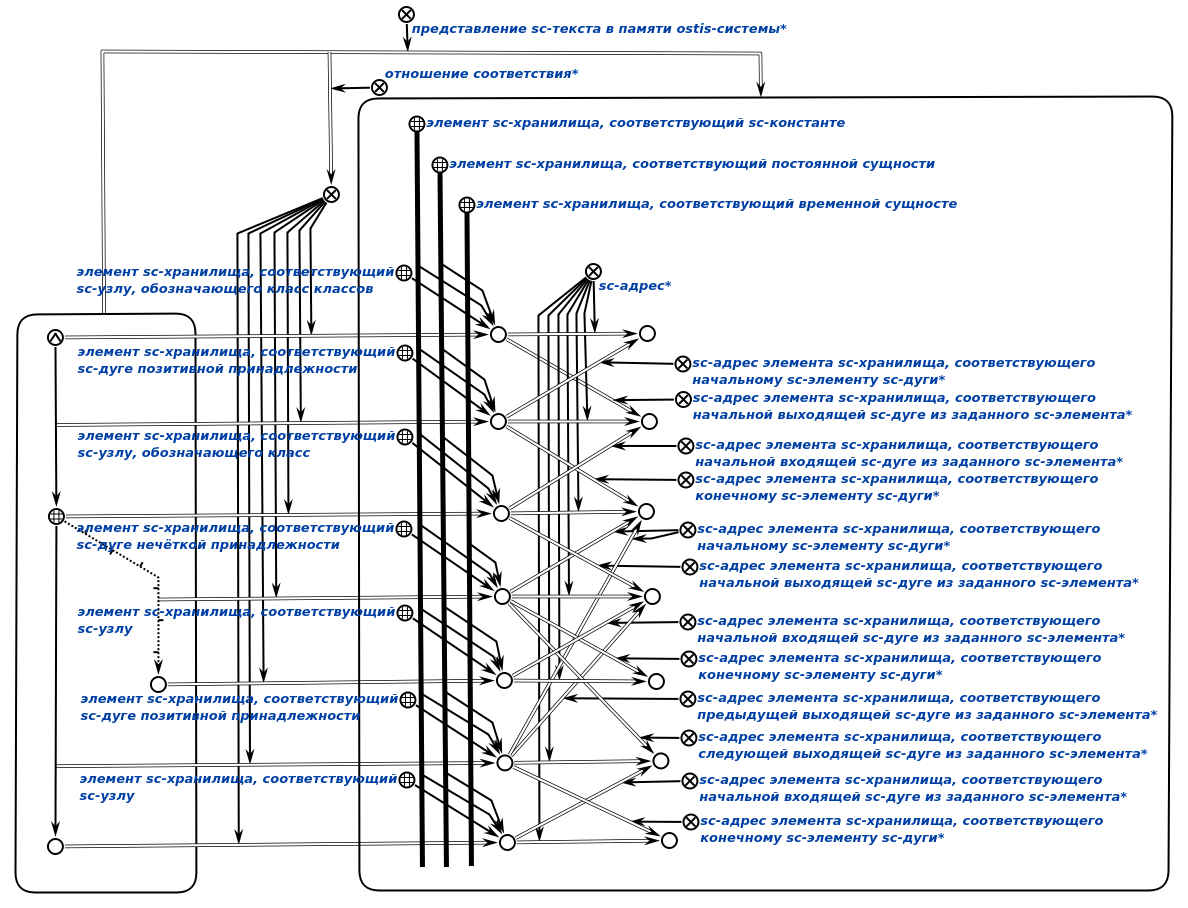
\includegraphics[scale=0.55]{author/part6/figures/sc_code_in_memory_representation.png}
  \caption{Пример спецификации представления конструкции SC-кода в памяти ostis-системы}
  \label{fig:sc_code_in_memory_representation}
\end{figure*}

Данная модель представления в памяти системы синтаксических и семантических классов sc-элементов в виде синтаксических и семантических классов элементов sc-элементов хранилища, которые соответствуют первым, обладает рядом преимуществ:
\begin{itemize}
    \item \textit{Синтаксические и семантические классы элементов sc-хранилища} могут комбинироваться между собой для получения более частных классов. С точки зрения программной реализации такая комбинация может быть представлена операцией побитового сложения значений соответствующих числовых выражений \textit{классов элементов sc-хранилища} (здесь, в спецификации на SC-коде это можно сделать с помощью пересечения соответствующих классов). Так, например, побитовое сложение числовых выражений классов элементов sc-хранилища, соотвествующих sc-узлу и sc-константе в результате образуют новый класс элементов sc-хранилища -- \textit{элемент sc-хранилища, соответствующий константному sc-узлу}.
    \item Числовые выражения некоторых классов могут совпадать. Это сделано для уменьшения размера элемента sc-хранилища за счет уменьшения максимального размера числового выражения класса этих элементов. Конфликт в данном случае не возникает, поскольку такие классы не могут комбинироваться, например \textit{элемент sc-хранилища, соответствующий sc-узлу ролевого отношения} и \textit{элемент sc-хранилища, соответствующий sc-дуге нечёткой принадлежности}.
    \item Важно отметить, что каждому из выделенных классов элементов (кроме классов, получаемых путем комбинации других классов) однозначно соответствует порядковый номер бита в линейной памяти, что можно заметить, глядя на соответствующие числовые выражения этих классов. Это означает, что классы элементов не включаются друг в друга (хоть в спецификации это и не так), например, указание принадлежности к классу \textit{элементов sc-хранилища, соответствующих sc-дуге позитивной принадлежности} не означает автоматическое указание принадлежности \textit{элементов sc-хранилища, соответствующих sc-дуге принадлежности}. На уровне реализации, это позволяет сделать операции комбинирования и сравнения меток более эффективными.
\end{itemize}

Sc-адрес никак не учитывается при обработке базы знаний на семантическом уровне и необходим только для обеспечения доступа к соответствующей структуре данных, хранящейся в линейной памяти на уровне \textit{Реализации sc-хранилища}.

В общем случае sc-адрес элемента sc-хранилища, соответствующего заданному sc-элементу, может меняться, например, при пересборке базы знаний из исходных текстов и последующем перезапуске системы. При этом sc-адрес элемента sc-хранилища, соответствующего заданному sc-элементу, непосредственно в процессе работы системы в текущей реализации меняться не может. Для простоты будем говорить \scnqq{sc-адрес sc-элемента}, имея в виду \textit{sc-адрес} \textit{элемента sc-хранилища}, однозначно соответствующего данному \textit{sc-элементу}.

В текущей \textit{Реализации sc-хранилища} \textit{классы уровня доступа} используются для того, чтобы обеспечить возможность ограничения доступа некоторых процессов в sc-памяти к некоторым элементам, хранимым в sc-памяти. Каждый элемент sc-хранилища принадлежит один из двух классов: классу \textit{элементов sc-хранилища, соответствующих sc-элементам, на которых разрешено право чтения} и классу \textit{элементов sc-хранилища, соответствующих sc-элементам, на которых разрешено право записи}. Каждая из которых выражается числом от 0 до 255.


Таким образом нулевое значение числовых выражений класса \textit{элементов sc-хранилища, соответствующих sc-элементам, на которых разрешено право чтения} и класса \textit{элементов sc-хранилища, соответствующих sc-элементам, на которых разрешено право записи} означает, что любой процесс может получить неограниченный доступ к данному элементу sc-хранилища.


Каждый элемент sc-хранилища, соответствующий некоторому sc-элементу, описывается его синтаксическим типом (меткой), а также независимо от типа указывается sc-адрес первой входящей в данный sc-элемент sc-дуги и первой выходящей из данного sc-элемента sc-дуги (могут быть пустыми, если таких sc-дуг нет). Оставшиеся байты в зависимости от типа соответствующего sc-элемента (sc-узел или sc-дуга) могут использоваться для хранения спецификации sc-дуги. Также \textit{sc-адрес первой sc-дуги, выходящей из данного sc-элемента*} и \textit{sc-адрес первой sc-дуги, входящей в данный sc-элемент*} в общем случае могут отсутствовать (быть нулевыми, \scnqq{пустыми}), но размер sc-элемента в байтах останется тем же.


С точки зрения программной реализации. структура данных для хранения sc-узла и sc-дуги остается остается та же, но в ней меняется список полей (компонентов). Кроме того, как можно заметить каждый элемент sc-хранилища (в том числе, \textit{элемент sc-хранилища, соответствующий sc-дуге}) не хранит список sc-адресов связанных с ним sc-элементов, а хранит sc-адреса одной выходящей и одной входящей дуги, каждая из которых в свою очередь хранит sc-адреса следующей и предыдущей дуг в списке исходящих и входящих sc-дуг для соответствующих элементов. Всё перечисленное позволяет:

\begin{itemize}
    \item сделать размер такой структуры фиксированным (в настоящее время 36 байт) и не зависящим от синтаксического типа хранимого sc-элемента;
    \item обеспечить возможность работы с sc-элементами без учета их синтаксического типа в случаях, когда это необходимо (например, при реализации поисковых запросов вида \scnqqi{Какие sc-элементы являются элементами данного множества}, \scnqqi{Какие sc-элементы непосредственно связаны с данным sc-элементом} и т.д.);
    \item обеспечить возможность доступа к \textit{элементу sc-хранилища} за константное время;
    \item обеспечить возможность помещения \textit{элемента sc-хранилища} в процессорный кэш, что в свою очередь, позволяет ускорить обработку sc-конструкций;
\end{itemize}

\section{Реализация файлового хранилища ostis-системы}

SC-код хоть и является универсальным средством для представления любых видов знаний, но не всегда есть необходимость погружать что-либо в графодинамическую память ostis-системы, по крайней мере, на ранних стадиях развития ostis-платформы. Это может быть объяснено и тем, что информационные конструкции, не принадлежащие SC-коду, достаточно сложны в синтаксисе и объёме. Для решения таких проблем на уровне \textit{Алфавита SC-кода\scnsupergroupsign} вводится дополнительный элемент -- внутренний файл ostis-системы. С помощью файлов ostis-системы можно представлять, хранить, обрабатывать и визуализировать информационные конструкции, не принадлежащие SC-коду, с помощью SC-кода.

Поэтому при реализации sc-памяти необходимо учитывать необходимость хранения информационных конструкций, не принадлежащих SC-коду, с помощью SC-кода. Таковым решением является \textit{Реализация файлового хранилища ostis-системы.}

За весь период развития \textit{Программного варианта реализации ostis-платформы} было достаточно много попыток реализовать полно функциональное и быстрое файловое хранилище на базе популярных баз данных. Однако из всех этих решений не было учтены потенциальные проблемы при реализации поисково-навигационной подсистемы \textit{Программного варианта реализации ostis-платформы}. Сейчас файловое хранилище реализовано своими средствами, в качестве структур данных для хранения информационных конструкций, не принадлежащих SC-коду, используются префиксные деревья \scncite{Bayer1977} и линейные списки.

Выбор аргументируется тем, что:
\begin{itemize}
    \item префиксные структуры достаточно просты в понимании и минимальны в своём синтаксисе;
    \item с помощью префиксных структур достаточно удобно хранить и обрабатывать связи типа \scnqq{ключ-значение};
    \item доступ к значению по ключу происходит в худшем случае за длину этого ключа \cite{tsuruta2022cPrefixTree}, \scncite{Belazzougui2010};
    \item за счёт того, что префиксы склеиваются, выходит сильный выигрыш в использовании памяти.
\end{itemize}

\begin{SCn}
\scnheader{Реализация файлового хранилища ostis-системы}
\scniselement{реализация файлового хранилища на основе префиксного дерева}
\scnrelto{программная модель}{файловое хранилище ostis-системы}
\scniselement{атомарный многократно используемый компонент ostis-систем}
\scniselement{зависимый многократно используемый компонент ostis-систем}
\begin{scnrelfromset}{зависимости компонента}
    \scnitem{Библиотека методов и структур данных GLib}
\end{scnrelfromset}
\begin{scnrelfromlist}{язык представления методов}
    \scnitem{C}
\end{scnrelfromlist}
\begin{scnrelfromlist}{внутренний язык}
    \scnitem{SCfin-код}
\end{scnrelfromlist}
\end{SCn}

\section{Формальная спецификация языка внутренного представления конструкций, не принадлежазщих SC-коду, в памяти ostis-системы}

Как в случае и с sc-хранилищем, необходимо описать язык представления информационных конструкций, не принадлежащих SC-коду, внутри файлового хранилища ostis-системы.

Такой язык будем называть языком внутренного представления информационных конструкций, не принадлежащих SC-коду, или, кратко, \textit{SCfin-кодом (Semantic Сode file interior)}. Файловое хранилище текстов, не принадлежащих SC-коду (как абстрактную модель, по которой можно реализововать соответствующее ей файловое хранилище платформы), можно рассматривать как подмножество scfin-текста.

\begin{SCn}
\scnheader{SCfin-код}
\scnidtf{Semantic Code file interior}
\scnidtf{Язык внутренного смыслового представления информационных конструкций, не принадлежащих SC-коду, внутри памяти ostis-системы}
\scnidtf{метаязык описания представления информационных конструкций, не принадлежащих SC-коду, внутри памяти ostis-системы}
\scntext{часто используемый неосновной внешний идентификатор sc-элемента}{scfin-текст}
\begin{scnindent}
    \scniselement{имя нарицательное}
\end{scnindent}
\scniselement{абстрактный язык}
\scniselement{метаязык}
\scnsubset{SC-код}
\scnsuperset{файловое хранилище ostis-системы}
\end{SCn}

\textit{Синтаксис SCfin-кода} задается: (1) \textit{Алфавитом SCfin-кода}, (2) отношением порядка \textit{последовательность в линейном тексте*}.

\begin{SCn}
\scnheader{Алфавит SCfin-кода\scnsupergroupsign}
\scnidtf{синтаксический тип элемента файлового хранилища ostis-системы}
\scnidtf{Множество типов элементов файлового хранилища ostis-системы}
\scnrelto{алфавит}{SCfin-код}
\begin{scneqtoset}
    \scnitem{элемент файлового хранилища ostis-системы, соответствующий подстроке текста линейного языка}
\end{scneqtoset}
\end{SCn}

\textit{Алфавит SCfin-кода\scnsupergroupsign} состоит из одного синтаксически выделяемого типа элементов файлового хранилища -- \textit{элемента файлового хранилища ostis-системы, соответствующего подстроке текста линейного языка}.

\begin{SCn}
\scnheader{элемент файлового хранилища ostis-системы, соответствующий подстроке текста линейного языка}
\scniselement{sc-элемент}
\scnidtf{элемент файлового хранилища}
\scnidtf{ячейка файлового хранилища}
\scnidtf{образ подстроки информационной конструкции, не принадлежащей SC-коду, в рамках файлового хранилища ostis-системы}
\end{SCn}

Отношение \textit{последовательности в линейном тексте*} определяется как бинарное ориентированное отношение порядка, компонентами каждой ориентированной пары которого является элементы файлового хранилища ostis-системы, соответствующие некоторым подстрокам линейного текста, в результате конкатенации которых образуется подстрока, принадлежащая этому же линейному тексту.

\textit{Синтаксис SCfin-кода} достаточно прост, поскольку информационные конструкции на нём задаются при помощи \textit{Алфавита SCfin-кода}, мощность которого равна 1, и единственного отношения инцидентности \textit{последовательности в линейном тексте*}. Иерархии синтаксических элементов как таковые не выделяются, поскольку в этом нет необходимости.

На уровне реализации важно выделить семантические классы э\textit{лементов файлового хранилища ostis-системы, соответствующий подстроке текста линейного языка}, которые обозначают некоторую префиксную или постфиксную часть целой информационной конструкции.

\begin{SCn}
\scnstructheader{Семантическая классификация элементов SCfin-кода}
\begin{scnsubstruct}

\scnheader{элемент файлового хранилища ostis-системы, соответствующий текста линейного языка}
\scnrelfrom{разбиение}{Типология элементов по месту расположения подстроки в линейном тексте}
\begin{scnindent}
    \begin{scneqtoset}
        \scnitem{элемент файлового хранилища ostis-системы, соответствующий префиксной подстроке текста линейного языка}
        \scnitem{элемент файлового хранилища ostis-системы, соответствующий постфиксной подстроке текста линейного языка}
    \end{scneqtoset}
\end{scnindent}

\end{scnsubstruct}
\end{SCn}

На SCfin-коде достаточно просто задавать информационные конструкции любых линейных текстов. Однако с точки зрения реализуемой модели sc-памяти есть необходимость задавать не столько форму информационных конструкций, не принадлежащих SC-коду, внутри файлового хранилища ostis-системы, сколько связи между этими внещними информационными конструкциями файлами ostis-системы, являющихся знаками SC-кода. Одновременно должны быть реализованы на уровне sc-памяти и метод получения файлов ostis-системы, которые содержат заданную внешнюю информационную конструкцию, и методы получения внешних информационных конструкций из заданных файлов ostis-системы.

На рисунке \nameref{fig:file_in_memory_representation} показано представление информационных конструкций, не принадлежащих SC-коду и соответствия между файлами ostis-системы и информационными конструкциями. С помощью отношения \textit{множество sc-адресов файлов ostis-системы по префиксам их содержимого*} задаётся бинарная ориентированная пара, первым компонентом которой является префиксная структура, элементами которой являются подстроки внешних информационных конструкций, а вторым компонентом -- множество соотвествующих им sc-адресов файлов ostis-системы, а с помощью отношения \textit{множество постфиксов содержимого файлов ostis-системы по их sc-адресам*} задаётся бинарная ориентированная пара, первым компонентом которой является префиксная структура, элементами которой являются подстроки sc-адресов файлов ostis-системы, представленных в строковом виде, а вторым компонентом -- множество соотвествующих им постфиксов внешних информационных конструкций префиксной структуры, являющейся первым компонентом каждой пары отношения \textit{множество sc-адресов файлов ostis-системы по префиксам их содержимого*}.

\begin{figure*}[htbp]
	\center
	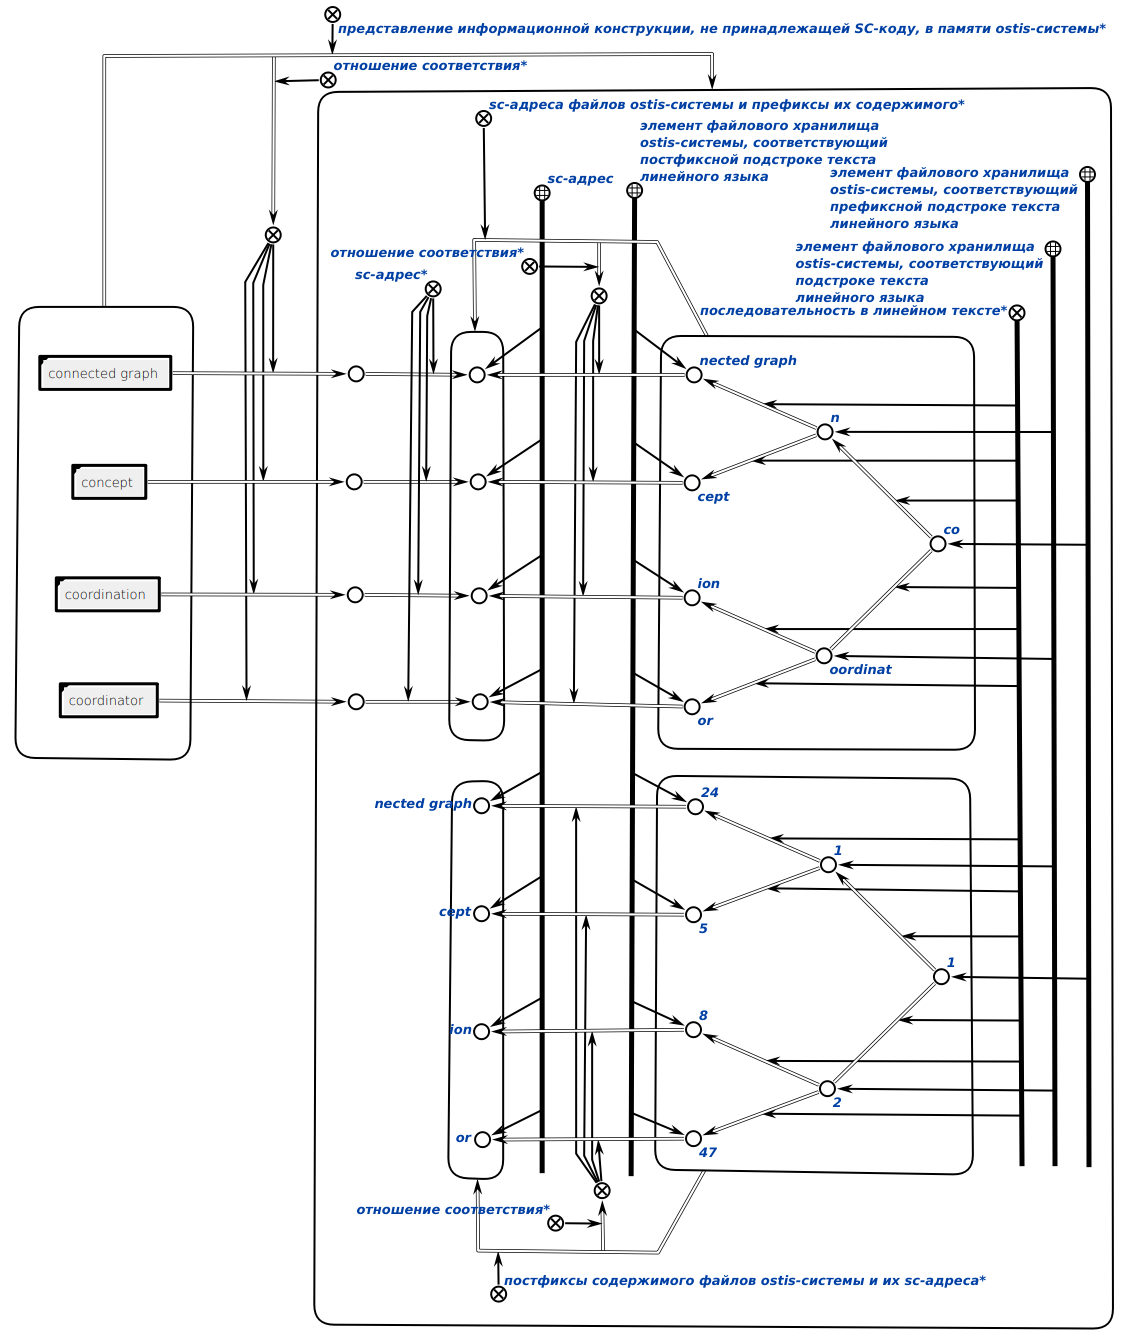
\includegraphics[scale=0.6]{author/part6/figures/file_in_memory_representation.png}
	\caption{Пример спецификации представления информационных конструкций, не принадлежащих SC-коду, в памяти ostis-системы}
	\label{fig:file_in_memory_representation}
\end{figure*}

Используемая \textit{Реализация файлового хранилища ostis-системы} полностью оправдывает себя при взаимодействии с системой. Благодаря использованию префиксных стуктур асимптотические сложности метода получения множества внешних информационных конструкций из заданных файлов ostis-системы и метода получения множества файлов ostis-системы по заданным внешним информационным конструкциям линейны, так как зависит от длины заданной строки и структуры префиксного дерева.

Среди общих недостатков данной \textit{Реализации файлового хранилища ostis-системы} можно выделить следующие:
\begin{itemize}
    \item Информационные конструкции, не принадлежащие SC-коду, пока полностью хранятся в оперативной памяти компьютерного устройства, на котором развёрнута платформа. Данную проблему можно решить, если в оперативной памяти хранить только первые знаки подстрок информационных конструкций, а остальные части этих подстрок хранить на уровне файлового системы.
    \item На данный момент информационно-поисковая подсистема реализована не полностью. \textit{Реализация файлового хранилища ostis-системы} позволяет быстро решать задачи поиска внешних информационных конструкций по их префиксным подстрокам, однако не позволяет быстро решать задачи поиска информационных конструкций по любой подстроке, даже для которого задан некоторый шаблон-образец.
\end{itemize}

Описанные проблемы будут решены в рамках будущей версии \textit{Программного варианта реализации ostis-платформы}.

\section{Реализация подсистема взаимодействия ostis-платформы с внешней средой}

В общем случае подсистема взаимодействия ostis-платформы с внешней средой может быть реализована по-разному. Так, например, до момента реализации текущей подсистемы ранее существовал её аналог на языке программирования Python, который использовал протокол HTTP и бинарное представление команд и ответов.
Поэтому можно говорить о большом разнообразии таких подсистем, которые будут составлять множество всевозможных \textit{Реализаций подсистемы взаимодействия с внешней средой с использованием сетевых языков}.

Данная \textit{Реализация подсистемы взаимодействия c sc-памятью на основе языка JSON} позволяет ostis-системам взаимодействовать с системами из внешней среды на основе общепринятого транспортного формата передачи данных JSON и предоставляет API для доступа к sc-памяти платформы интерпретации sc-моделей.

\begin{SCn}
\scnheader{Реализация подсистемы взаимодействия с внешней средой с использованием сетевых языков}
\begin{scnrelfromset}{декомпозиция программной системы}
    \scnitem{Реализация подсистемы взаимодействия с внешней средой с использованием сетевых языков на основе языка JSON}
\end{scnrelfromset}
\end{SCn}

\begin{SCn}
\scnheader{Реализация подсистемы взаимодействия c sc-памятью на основе языка JSON}
\scnidtf{Подсистема взаимодействия с sc-памятью на основе формата JSON}
\scniselement{неатомарный многократно используемый компонент ostis-систем}
\scniselement{зависимый многократно используемый компонент ostis-систем}
\scniselement{клиент-серверная система}
\begin{scnrelfromlist}{используемый язык представления методов}
    \scnitem{C}
    \scnitem{C++}
    \scnitem{Python}
    \scnitem{TypeScript}
    \scnitem{C\#}
    \scnitem{Java}
\end{scnrelfromlist}
\begin{scnrelfromlist}{используемый язык}
    \scnitem{SC-JSON-код}
\end{scnrelfromlist}
\begin{scnrelfromset}{декомпозиция программной системы}
    \scnitem{Серверная система на основе Websocket и JSON, обеспечивающая сетевой доступ к sc-памяти}
    \scnnonamednode
    \begin{scneqtoset}
        \scnitem{Реализация клиентской системы на языке программирования Python}
        \scnitem{Реализация клиентской системы на языке программирования TypeScript}
        \scnitem{Реализация клиентской системы на языке программирования C\#}
        \scnitem{Реализация клиентской системы на языке программирования Java}
    \end{scneqtoset}
\end{scnrelfromset}
\end{SCn}

Взаимодействие c sc-памятью обеспечивается с помощью передачи информации на \textit{SC-JSON-коде} и ведётся, с одной стороны, между сервером, являющегося частью ostis-системы, написанным на том же языке реализации этой ostis-системы и имеющим доступ к её sc-памяти, и с другой стороны множеством клиентоd, которым известно о наличии сервера в пределах сети их использования. С помощью подсистемы взаимодействия с sc-памятью на основе языка JSON можно взаимодействовать с ostis-системой на таком же множестве возможных операций, как и в случае, если бы взаимодействие происходило (непосредственно) напрямую, на том же языке реализации платформы интерпретации sc-моделей компьютерных систем. При этом результат работы отличается только скоростью обработки информации.
Взаимодействие программной модели sc-памяти с внешними ресурсами может осуществляться посредством специализированного программного интерфейса (API), однако этот вариант неудобен в большинстве случае, поскольку:
    \begin{itemize}
        \item поддерживается только для очень ограниченного набора языков программирования;
        \item требует того, чтобы клиентское приложение, обращающееся к программной модели sc-памяти, фактически составляло с ней единое целое, таким образом исключается возможность построения распределенного коллектива ostis-систем;
        \item как следствие предыдущего пункта, исключается возможность параллельной работы с sc-памятью нескольких клиентских приложений.
   \end{itemize}
Для того, чтобы обеспечить возможность удаленного доступа к sc-памяти не учитывая при этом языки программирования, с помощью которых реализовано конкретное клиентское приложение, было принято решение о реализации возможности доступа к sc-памяти с использованием универсального языка, не зависящего от средств реализации того или иного компонента или системы.

Среди эффективных протоколов, используемых при реализации клиент-серверных систем, стоит отметить протоколы прикладного уровня стека TCP/IP -- протоколы HTTP и WebSocket \cite{webockets_overview}, \cite{naik2020study}. Целесообразным является использование протокола WebSocket, это объясняется следующими причинами:

\begin{itemize}
    \item WebSocket выгодно использовать в веб-ориентированных системах, в которых данные, отправляемые сервером, представляются или сохраняются на стороне клиента. В WebSocket данные постоянно передаются через одно и то же открытое соединение, поэтому коммуникация по протоколу WebSocket быстрее чем коммуникация по HTTP \scncite{Tomasetti2021}, \cite{webockets_overview}. Это очень важно с точки зрения проектирования Экосистемы OSTIS, которые могут состоять из десятков тысяч различного вида ostis-систем.
    \item Поскольку в основе ostis-систем лежит идея агентно-ориентированной обработки знаний (асинхронной обработки), а память таких систем должна быть одновременно распределённой и общей, то необходимо, чтобы каждая из них (в частности, самостоятельная ostis-система) могла общаться с другими ostis-системами. Причём такое общение может и должно происходить на условиях иницирования событий в памяти этих систем. Отсюда следует однозначный вывод, что протокол HTTP не может быть использован в передовых интеллектуальных системах нового поколения по причине однонаправленности создаваемого им соединения.
\end{itemize}
В качестве языка коммуникации систем был разработан строковый язык на базе языка JSON \cite{pezoa2016foundations}, \scncite{Marrs2017} -- SC-JSON-код. Его выбор объясняется гибкостью задания отношений между описываемыми им объектами.

Как говорилось ранее, подсистемы в рамках реализуемого программного варианта специализированной платформы общаются с помощью языка внешнего представления знаний SC-JSON-код. Данный язык является строковым, то есть линейным, и легкообратаваемым, поскольку существует большое количество средств для обработки его надъязыка JSON.

\begin{SCn}
\scnheader{SC-JSON-код}
\scnidtf{Semantic JSON-code}
\scnidtf{Semantic JavaScript Object Notation code}
\scnidtf{Язык внешнего смыслового представления знаний на основе языка JSON}
\scntext{часто используемый неосновной внешний идентификатор sc-элемента}{sc-json-текст}
\begin{scnindent}
    \scniselement{имя нарицательное}
\end{scnindent}
\scniselement{абстрактный язык}
\scniselement{линейный язык}
\scnsubset{JSON}
\end{SCn}

\textit{Синтаксис SC-JSON-кода} задается: (1) \textit{Алфавитом SC-JSON-кода}, (2) Грамматикой SC-JSON-кода. В алфавите SC-JSON-кода выделяется базовая синтаксическая классификация его элементов.

\begin{SCn}
\scnstructheader{Синтаксическая классификация элементов SC-JSON-кода}

\begin{scnsubstruct}
\scnstructheader{SC-JSON-код}
\scnrelto{семейство подмножеств}{sc-json-предложение}
\begin{scnindent}
    \scnsubset{json-список json-пар}
    \scnrelto{семейство подмножеств}{sc-json-пара*}
    \begin{scnindent}
        \begin{scnreltovector}{декартово произведение}
            \scnitem{sc-json-строка}
            \scnitem{sc-json-объект}
        \end{scnreltovector}
    \end{scnindent}
    \begin{scnrelfromset}{разбиение}
        \scnitem{команда на SC-JSON-коде}
        \scnitem{ответ на команду на SC-JSON-коде}
    \end{scnrelfromset}
\end{scnindent}

\scnheader{sc-json-объект}
\begin{scnrelfromset}{разбиение}
    \scnitem{sc-json-cписок}
    \scnitem{sc-json-пара}
    \scnitem{sc-json-литерал}
    \begin{scnindent}
        \begin{scnrelfromset}{разбиение}
            \scnitem{sc-json-строка}
            \scnitem{sc-json-число}
        \end{scnrelfromset}
    \end{scnindent}
\end{scnrelfromset}
\end{scnsubstruct}
\end{SCn}

\textit{Алфавит SC-JSON-кода\scnsupergroupsign} представляет собой множество всех возможных символов в SC-JSON-коде. Поскольку \textit{SC-JSON-код} является линейным строковым языком представления знаний, то его алфавит включает объединение алфавитов всех языков, тексты на которых могут представлять внешние идентификаторы и/или содержимое файлов ostis-системы, множество всех цифр и множество всех других специальных символов. Последовательности знаков алфавита могут образовывать sc-json ключевые слова, \textit{sc-json-пары}, \textit{sc-json-предложения} из \textit{sc-json-пар} и \textit{sc-json-тексты} из \textit{sc-json-предложений}. При этом конструкции на SC-JSON-коде строятся по следующим синтаксическим правилам:
\begin{itemize}
    \item Каждое правило \textit{Грамматики SC-JSON-кода} описывает корректный с точки зрения \textit{Синтаксиса SC-JSON-кода} порядок sc-json-объектов в sc-json-предложении. Совокупность правил \textit{Грамматики SC-JSON-кода} описывает корректный с точки зрения \textit{Синтаксиса SC-JSON-кода} порядок sc-json-предложений в sc-json-тексте. Каждое sc-json-предложение является sc-json-списком, состоящим из sc-json-пар и представляет собой команду или ответ на эту команду.
    \item Каждая \textit{команда (ответ на команду) на SC-JSON-коде} состоит из заголовка, включающего sc-json-пары описания самой команды (ответа на команду), и сообщения, различного для каждого класса команд (ответов на команды). Сообщение \textit{команды (ответа на команду) на SC-JSON-коде} обычно представляет собой список sc-json-объектов и может не ограничиваться по мощности.
    \item Каждая sc-json-пара состоит из двух элементов: ключевого слова и некоторого другого sc-json-объекта, ассоциируемого с этим ключевым словом. Набор ключевых слов в sc-json-парах определяется конкретным классом \textit{команд (ответов на команды) на SC-JSON-коде}. Sc-json-пара начинается знаком открывающейся фигурной скобки \scnqq{\{} и заканчивается знаком закрывающейся фигурной скобки \scnqq{\}}. Ключевое слово и sc-json-объект, ассоциируемый с ним, разделяются при помощи знака двоеточия \scnqq{:}.
    \item Sc-json-строки, записанные в sc-json-текстах, начинаются и заканчиваются знаком двух ковычек \textquotedblleft.
    \item Sc-json-списки, состоящие не из sc-json-пар, начинаются знаком открывающейся квадратной скобки \scnqq{[} и заканчиваются знаком закрывающейся квадратной скобки \scnqq{]}. Sc-json-объекты в sc-json-списках разделяются запятыми \scnqq{,}.
\end{itemize}

Грамматика SC-JSON-кода представляет собой множество всех возможных правил, используемых при построении команд и ответов на них на SC-JSON-коде. Каждой команде \textit{SC-JSON-кода} однозначно соответствует правило грамматики \textit{SC-JSON-кода}. Правила \textit{Грамматики SC-JSON-кода} позволяют правильно представлять команды на SC-JSON-коде. Каждое правило грамматики \textit{SC-JSON-кода} представляется в виде правила на \textit{Языке описания грамматик ANTLR} и его интерпретации на естественном языке.

\begin{SCn}
\scnheader{Грамматика SC-JSON-кода}
\scnhaselementrole{ключевой sc-элемент}{Правило, задающее синтаксис \textit{команд на SC-JSON-коде}}
\begin{scnindent}
    \scnrelto{синтаксическое правило}{команда на SC-JSON-коде}
\end{scnindent}
\scnhaselementrole{ключевой sc-элемент}{Правило, задающее синтаксис \textit{ответов на команды на SC-JSON-коде}}
\begin{scnindent}
    \scnrelto{синтаксическое правило}{ответ на команду на SC-JSON-коде}
\end{scnindent}
\scnhaselement{Правило, задающее синтаксис \textit{команды создания sc-элементов}}
\begin{scnindent}
    \scnrelto{синтаксическое правило}{команда создания sc-элементов}
\end{scnindent}
\scnhaselement{Правило, задающее синтаксис \textit{ответа на команду создания sc-элементов}}
\begin{scnindent}
    \scnrelto{синтаксическое правило}{ответ на команду создания sc-элементов}
\end{scnindent}
\end{SCn}

Правило, задающее синтаксис \textit{команд на SC-JSON-коде} представлено на рисунке \nameref{fig:command}. Класс \textit{команд на SC-JSON-коде} включает \textit{команду создания sc-элементов}, \textit{команду получения соответствующих типов sc-элементов}, \textit{команду удаления sc-элементов}, \textit{команду обработки ключевых sc-элементов}, \textit{команду обработки содержимого файлов ostis-системы}, \textit{команду поиска sc-конструкций, изоморфных заданному sc-шаблону}, \textit{команду генерации sc-конструкции, изоморфной заданному sc-шаблону}, и \textit{команду обработки sc-событий}. В \textit{команду на SC-JSON-коде} включаются идентификатор этой команды, тип и сообщение.

\begin{figure}[htbp]
  \center
  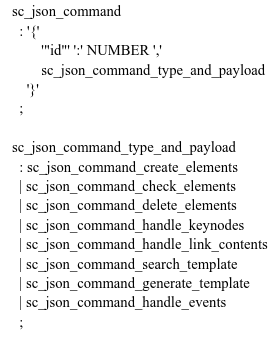
\includegraphics[scale=0.9]{author/part6/figures/command.png}
  \caption{Описание Правила, задающего синтаксис \textit{команд на SC-JSON-коде}}
  \label{fig:command}
\end{figure}

Правило, задающее синтаксис \textit{ответа на команду на SC-JSON-коде} описывает синтаксис ответов на команды, описываемых предыдущим правилом. Класс \textit{ответов на команды на SC-JSON-коде} включает \textit{ответ на команду создания sc-элементов}, \textit{ответ на команду получения соответствующих типов sc-элементов}, \textit{ответ на команду удаления sc-элементов}, \textit{ответ на команду обработки ключевых sc-элементов}, \textit{ответ на команду обработки содержимого файлов ostis-системы}, \textit{ответ на команду поиска sc-конструкций, изоморфных заданному sc-шаблону}, \textit{ответ на команду генерации sc-конструкции, изоморфной заданному sc-шаблону}, и \textit{ответ на команду обработки sc-событий}. В \textit{ответ на команду на SC-JSON-коде} включаются идентификатор соответствующей команды, статус обработки ответа и ответное сообщение \nameref{fig:command_answer}.

\begin{figure}[htbp]
  \center
  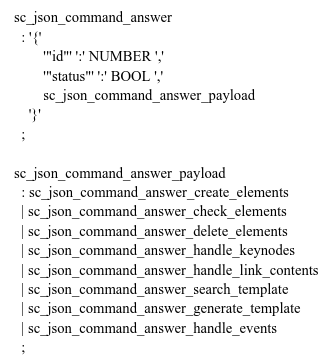
\includegraphics[scale=0.8]{author/part6/figures/command_answer.png}
  \caption{Описание Правила, задающего синтаксис \textit{ответов на команды SC-JSON-кода}}
  \label{fig:command_answer}
\end{figure}

В сообщении \textit{команды создания sc-элементов} представляется список описаний создаваемых sc-элементов. Такими sc-элементами могут быть sc-узел, sc-дуга, sc-ребро или файл ostis-системы. Тип sc-элемента указывается в паре с ключевым словом \scnqq{el}: для sc-узла sc-json-тип элемента представляется как \scnqq{node}, для sc-дуги и sc-ребра -- \scnqq{edge}, для файла ostis-системы -- \scnqq{link}. Метки типов sc-элементов уточняются в соответствующих им описаниях в сообщении команды в паре с ключевым словом \scnqq{type}. Если создаваемым sc-элементом является файл ostis-системы, то дополнительно указывается содержимое этого файла ostis-системы в паре с ключевым словом \scnqq{content}, если создаваемым sc-элементом является sc-дуга или sc-ребро, то указываются описания sc-элементов, из которых они выходят, и sc-элементов, в которые они входят. Описание таких sc-элементов состоят из двух пар: первая пара указывает на способ ассоциации с sc-элементом и представляется как \scnqq{addr} или \scnqq{idtf} или \scnqq{ref} в паре с ключевым словом \scnqq{type}, вторая пара -- то, по чему происходит ассоциация с этим sc-элементом: его хэшу, системному идентификатору или номеру в массиве создаваемых sc-элементов -- в паре с ключевым словом \scnqq{value} \nameref{fig:create_elements_command}.

\begin{figure}[htbp]
	\center
	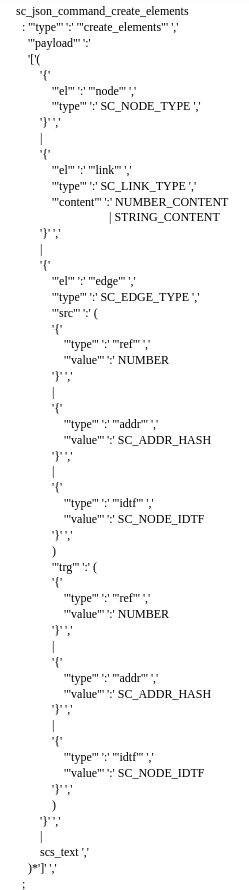
\includegraphics[scale=0.8]{author/part6/figures/create_elements_command.png}
	\caption{Описание Правила, задающего синтаксис \textit{команды создания sc-элементов}}
	\label{fig:create_elements_command}
\end{figure}

Сообщением \textit{ответа на команду создания sc-элементов} является список хэшей созданных sc-элементов, соответствующих описаниям \textit{команды создания sc-элементов} со статусом 1, в случае успешной обработки команды \nameref{fig:create_elements_command_answer}.

\begin{figure}[htbp]
	\center
	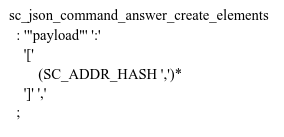
\includegraphics[scale=0.8]{author/part6/figures/create_elements_command_answer.png}
	\caption{Описание Правила, задающего синтаксис \textit{ответа на команду создания sc-элементов}}
	\label{fig:create_elements_command_answer}
\end{figure}

Множество \textit{команд на SC-JSON-коде} легко расширяемо засчёт гибкости и функциональности языка JSON. Множество \textit{ответов на команды на SC-JSON-коде} также легко расширяемо вместе с расширением \textit{команд на SC-JSON-коде}.

Детальное описание синтаксиса команд и ответов на эти команды, а также их примеры можно найти в Стандарте OSTIS \cite{Standard2021}.

\textit{Серверная система на основе Websocket и JSON, обеспечивающая сетевой доступ к sc-памяти}, представляет собой интерпретатор команд и ответов на них \textit{SC-JSON-кода} на программное представление sc-конструкций в sc-памяти при помощи \textit{Библиотеки программных компонентов для обработки json-текстов JSON for Modern C++} и \textit{Библиотеки кросс-платформенных программных компонентов для реализации серверных приложений на основе Websocket WebSocket++}, а также обеспечивается комплексным тестовым покрытием посредством программных фреймворков Google Tests и Google Benchmark Tests. \textit{Библиотека программных компонентов для обработки json-текстов JSON for Modern C++} имеет богатый, удобный и быстродействующий функционал, необходимый для реализации подобных компонентов ostis-систем, а \textit{Библиотека кросс-платформенных программных компонентов для реализации серверных приложений на основе Websocket WebSocket++} позволяет элегантно проектировать серверные системы без использовании избыточных зависимостей и решений. Настройка программного компонента осуществляется с помощью \textit{Программного компонента настройки программных компонентов ostis-систем} и скриптов языков CMake и Bash.

\begin{SCn}
\scnheader{Реализация Серверной системы на основе Websocket и JSON, обеспечивающей сетевой доступ к sc-памяти}
\scnidtf{Реализация системы, работающей по принципам Websocket и предоставляющая параллельно-асинхронный многоклиентский доступ к sc-памяти платформы интерпретации sc-моделей при помощи SC-JSON-кода}
\scnidtf{sc-json-сервер}
\scntext{часто используемый неосновной внешний идентификатор sc-элемента}{sc-сервер}
\scniselement{атомарный многократно используемый компонент ostis-систем}
\scniselement{зависимый многократно используемый компонент ostis-систем}
\begin{scnrelfromlist}{используемый язык представления методов}
    \scnitem{C}
    \scnitem{C++}
\end{scnrelfromlist}
\begin{scnrelfromlist}{используемый язык}
    \scnitem{SC-JSON-код}
\end{scnrelfromlist}
\begin{scnrelfromset}{зависимости компонента}
    \scnitem{Библиотека программных компонентов для обработки json-текстов JSON for Modern C++}
    \scnitem{Библиотека кросс-платформенных программных компонентов для реализации серверных приложений на основе Websocket WebSocket++}
    \scnitem{Программный компонент настройки программных компонентов ostis-систем версия}
    \scnitem{Реализация sc-памяти}
\end{scnrelfromset}
\end{SCn}

Стоит отметить, что текущая \textit{Реализация серверной системы на основе Websocket и JSON, обеспечивающей сетевой доступ к sc-памяти}, не является первой в своём роде и заменяет предыдущую ее реализацию, написанную на языке Python.
Причиной такой замены состоит в следующем:
\begin{itemize}
    \item предыдущая \textit{Реализация серверной системы на основе Websocket, обеспечивающей доступ к sc-памяти при помощи команд SC-JSON-кода}, реализованная на языке программирования Python, зависит от библиотеки Boost Python, предоставляемой сообществом по развитию и коллаборации языков С++ и Python. Дело в том, что такое решение требует поддержки механизма интерпретации программного кода на языке Python на язык С++, что является избыточным и необоснованным, поскольку большая часть программного кода \textit{Программного варианта реализации ostis-платформы} реализована на языках С и С++. Новая реализация описываемой программной системы позволяет избавиться от использования ёмких и ресурсозатратных библиотек(например, boost-python-lib, llvm) и языка Python;
    \item при реализации распределённых подсистем важную роль играет скорость обработки знаний, то есть возможность быстро и своевременно отвечать на запросы пользователя. Качество доступа к sc-памяти посредством реализованной \textit{Подсистемы взаимодействия с sc-памятью на основе языка JSON} должно быть соизмеримо с качеством доступа к sc-памяти при помощи специализированного программного интерфейса API, реализованного на том же языке программирования, что и сама система. Новая реализация позволяет повысить скорость обработки запросов \textit{Подсистемой взаимодействия с sc-памятью на основе языка JSON}, в том числе и обработка знаний, не менее чем в 1,5 раза по сравнению с предыдущим вариантом реализации этой подсистемы.
\end{itemize}

\textit{Реализация Серверной системы на основе Websocket и JSON, обеспечивающей сетевой доступ к sc-памяти}, обладает следующими общими характеристиками:
\begin{itemize}
    \item С точки зрения своей модели, серверная подсистема имеет такой же специализированный программный интерфейс, как и \textit{Реализация sc-памяти}, однако взаимодействие с ней при помощи такого интерфейса осуществляется посредством сети. Это обеспечивает возможность взаимодействия клиентских систем, реализованных на разных языкаъ программирования, с одной общей памятью.
    \item Данную подсистему можно рассматривать как некоторый интерпретатор внешнего языка представления знаний SC-JSON-код, на котором могут общаться ostis-системы, реализованные на базе специализированной ostis-платформы. Каждой команде и ответу на команду этого языка соответствует обработчик (потенциально и вовсе агент), который является частью этого интерпретатора. Сам язык внешнего представления знаний SC-JSON-код независим от реализации платформы и используется только как язык внешнего представления знаний, но может быть задействован при реализации других средств и интерпретаторов sc-моделей ostis-систем.
    \item Реализованный программный компонент предоставляет многопользовательский асинхронный доступ к sc-памяти. В ходе тестирования sc-сервера выяснилось, что его реализация позволяет обрабатывать запросы не менее чем 1000 клиентских систем. В связи с необходимостью обеспечения параллельного доступа к sc-памяти на уровне реализации программного компонента были добавлены блоки синхронизации. Например, в реализации можно заметить очередь команд на обработку системой -- вне зависимости от количества клиентских систем и того, в каком количестве они отправляют команды на обработку, все команды могут становиться в очередь. Такое решение позволяет временно обойти проблемы взаимодействия блоков синхронизации на уровне sc-памяти при обработки разных типов команд над ней (поисковых, генеративных, деструктивных и т. д.). При этом серверную систему невозможно отключить до тех пор, пока очередь команд имеет какие-нибудь необработанные команды. Также серверная система продолжает работать, если в списке идентификаторов клиентских систем остались неотключенные из них. Необходимость данных функций серверной подсистемы обуславливается необходимостью поддержки атомарности запросов, обрабатываемых системой.
    \item В процессе тестирования подсистемы были получена оценка её скорости обработки команд и ответов. При нагрузочном тестировании использовалась тестовая клиентская система, написанная на С++ и не имеющая функционала обработки текстов SC-JSON-кода. В результате тестирования было выяснено, что при отправке 1000 различных команд: команд создания sc-элементов, команд обработки содержимого файлов ostis-системы и команд удаления sc-элементов -- время, потраченное на их обработку не превышало 0,2 секунды. При этом в отдельных случаях на обработку 1000 команд создания sc-элементов уходило не более 0,14 секунды, команд удаления sc-элементов -- не более 0,07 секунды, команд обработки содержимого файлов ostis-системы -- не более 0,27 секунды, команд поиска sc-конструкций, изоморфных заданному sc-шаблону -- не более 0,45 секунды.
\end{itemize}

\textit{Серверная система на основе Websocket и JSON, обеспечивающая сетевой доступ к sc-памяти} описывает необходимый и достаточный программный интерфейс для взаимодействия c sc-памятью. В общем случае описывает функциональные возможности не только \textit{Серверной системы на основе Websocket, обеспечивающей доступ к sc-памяти платформы интерпретации sc-моделей при помощи команд SC-JSON-кода}, но и клиентских систем взаимодействующих с ней, поскольку зачастую эти клиентские системы включают специализированный программный интерфейс, схожий с интерфейсом серверной системы, но реализованный на другом языке программирования.

\section{Реализация интерпретатора sc-моделей пользовательских интерфейсов}

В большинстве случаев разработка пользовательского интерфейса в современных системах отнимает большую часть времени, затрачиваемого на разработку всей системы. Однако эффективность использования программной системы зависит от разрабатываемого пользовательского интерфейса \cite{Myers1992}.

Наряду с \textit{Реализацией sc-памяти} важной частью \textit{Программного варианта реализации ostis-платформы} является \textit{Реализация интерпретатора sc-моделей пользовательских интерфейсов}, которая предоставляет базовые средства просмотра и редактирования базы знаний пользователем, средства для навигации по базе знаний (задания вопросов к базе знаний) и может дополняться новыми компонентами в зависимости от задач, решаемых каждой конкретной ostis-системой.

\begin{SCn}
	\scnheader{Реализация интерпретатора sc-моделей пользовательских интерфейсов}
	\scniselement{неатомарный многократно используемый компонент ostis-систем}
	\scniselement{зависимый многократно используемый компонент ostis-систем}
	\begin{scnrelfromlist}{используемый язык представления методов}
		\scnitem{JavaScript}
		\scnitem{TypeScript}
		\scnitem{Python}
		\scnitem{HTML}
		\scnitem{CSS}
	\end{scnrelfromlist}
	\begin{scnrelfromset}{зависимости компонента}
		\scnitem{Библиотека стандартных интерфейсных компонентов на языке программирования JavaScript}
		\scnitem{Библиотека для реализации серверных приложений на языке программирования Python Tornado}
		\scnitem{Реализация клиентской системы на языке программирования TypeScript}
		\scnitem{Реализация клиентской системы на языке программирования Python}
	\end{scnrelfromset}
\end{SCn}

Важным принципом \textit{Реализации интерпретатора sc-моделей пользовательских интерфейсов} является простота и однотипность подключения любых компонентов пользовательского интерфейса (редакторов, визуализаторов, переключателей, команд меню и т.д.). Для этого реализуется программная прослойка Sandbox, в рамках которой реализуются низкоуровневые операции взаимодействия с серверной частью и которая обеспечивает более удобный программный интерфейс для разработчиков компонентов. Текущий вариант \textit{Реализации интерпретатора sc-моделей пользовательских интерфейсов} является открытым и доступен на \cite{sc-web}.

\subsection{Основные компоненты интерпретатора sc-моделей пользовательских интерфейсов}

\begin{SCn}
	\scnheader{Реализация интерпретатора sc-моделей пользовательских интерфейсов}
	\begin{scnrelfromset}{декомпозиция программной системы}
		\scnitem{Панель меню команд пользовательского интерфейса}
		\scnitem{Компонент переключения языка идентификации отображаемых sc-элементов}
		\scnitem{Компонент переключения внешнего языка визуализации знаний}
		\scnitem{Поле поиска sc-элементов по идентификатору}
		\scnitem{Панель отображения диалога пользователя с ostis-системой}
		\scnitem{Панель визуализации и редактирования знаний}
		\begin{scnindent}
			\begin{scnrelfromset}{декомпозиция программной системы}
				\scnitem{Визуализатор sc.n-текстов}
				\scnitem{Визуализатор и редактор sc.g-текстов}
			\end{scnrelfromset}
		\end{scnindent}
	\end{scnrelfromset}
\end{SCn}

\textit{Компонент переключения языка идентификации отображаемых sc-элементов} является изображением множества имеющихся в системе естественных языков. Взаимодействие пользователя с данным компонентом переключает пользовательский интерфейс в режим общения с конкретным пользователем с использованием \textit{основных sc-идентификаторов}, принадлежащих данному \textit{естественному языку}. Это значит, что при изображении sc-идентификаторов sc-элементов на каком-либо языке, например, SCg-коде или SCn-коде будут использоваться \textit{основные sc-идентификаторы}, принадлежащие данному \textit{естественному языку}. Это касается как sc-элементов, отображаемых в рамках \textit{Панели визуализации и редактирования знаний}, так и любых других sc-элементов, например, классов команд и даже самих \textit{естественных языков}, изображаемых в рамках самого \textit{Компонента переключения языка идентификации отображаемых sc-элементов}.

\textit{Компонент переключения внешнего языка визуализации знаний} служит для переключения языка визуализации знаний в текущем окне, отображаемом на \textit{Панели визуализации и редактирования знаний}. В текущей реализации в качестве таких языков по умолчанию поддерживаются SCg-код и SCn-код, а также любые другие языки, входящие во множество \textit{внешних языков визуализации SC-кода}.

\textit{Поле поиска sc-элементов по идентификатору} позволяет осуществлять поиск \mbox{sc-идентификаторов}, содержащих подстроку, введенную в данное поле (с учетом регистра). В результате поиска отображается список sc-идентификаторов, содержащих указанную подстроку, при взаимодействии с которыми осуществляется автоматическое задание вопроса \scnqqi{Что это такое?}, аргументом которого является либо для сам sc-элемент, имеющий данный sc-идентификатор (в случае, если указанный sc-идентификатор является основным или системным, и, таким образом, указанный sc-элемент может быть определен однозначно), либо для самого внутреннего файла ostis-системы, являющегося sc-идентификатором (в случае, если данный sc-идентификатор является неосновным).

\textit{Панель отображения диалога пользователя с ostis-системой} отображает упорядоченный по времени список sc-элементов, являющихся знаками действий, которые инициировал пользователь в рамках диалога с ostis-системой путем взаимодействия с изображениями соответствующих классов команд (то есть, если действие было инициировано другим способом, например, путем его явного инициирования через создание дуги принадлежности множеству \textit{инициированных действий} в sc.g-редакторе, то на данной панели оно отображено не будет). При взаимодействии пользователя с любым из изображенных знаков действий на \textit{Панели визуализации и редактирования знаний} отображается окно, содержащее результат выполнения данного \textit{действия} на том языке визуализации, на котором он был отображен, когда пользователь просматривал его в последний (предыдущий) раз. Таким образом, в текущей реализации данная панель может работать только в том случае, если инициированное пользователем действие предполагает явно представленный в памяти результат данного действия. В свою очередь, из этого следует, что в настоящее время данная панель, как и в целом \textit{Реализация интерпретатора sc-моделей пользовательских интерфейсов}, позволяет работать с системой только в режиме диалога \scnqqi{вопрос-ответ}.

\textit{Панель визуализации и редактирования знаний} отображает окна, содержащие sc-текст, представленный на некотором языке из множества \textit{внешних языков визуализации SC-кода} и, как правило, являющийся результатом некоторого действия, инициированного пользователем. Если соответствующий визуализатор поддерживает возможность редактирования текстов соответствующего естественного языка, то он одновременно является также и редактором. При необходимости пользовательский интерфейс каждой конкретной ostis-системы может быть дополнен визуализаторами и редакторами различных внешних языков, которые в текущей версии \textit{Реализации интерпретатора sc-моделей пользовательских интерфейсов} будут также располагаться на \textit{Панели визуализации и редактирования знаний}. По умолчанию доступны две панели визуализации и редактирования: Визуализатор sc.n-текстов и Визулизатор и редактор sc.g-текстов.

\textit{Панель меню команд пользовательского интерфейса} содержит изображения классов команд (как атомарных, так и неатомарных), имеющихся на данный момент в базе знаний и входящих в декомпозицию \textit{Главного меню пользовательского интерфейса} (имеется в виду полная декомпозиция, которая в общем случае может включать несколько уровней неатомарных классов команд). Взаимодействие с изображением неатомарного класса команд инициирует команду изображения классов команд, входящих в декомпозицию данного неатомарного класса команд. Взаимодействие с изображением атомарного класса команд инициирует генерацию команды данного класса с ранее выбранными аргументами на основе соответствующей \textit{обобщенной формулировки класса команд} (шаблона класса команд).

Семантические модели описанных компонентов пользовательского интерфейса более подробно представлены в работе \cite{sadouski2022semantic}.

Текущая реализация интерпретатора sc-моделей пользовательских интерфейсов имеет большое множество недостатков, а именно:
\begin{itemize}
	\item Идея платформенной независимости пользовательского интерфейса (построения sc-модели пользовательского интерфейса) реализована не в полной мере. Полностью описать sc-модель пользовательского интерфейса (включая точное размещение, размеры, дизайн компонентов, их поведение и др.) в настоящее время скорее всего окажется затруднительно из-за ограничений производительности, однако вполне возможно реализовать возможность задания вопросов ко всем компонентам интерфейса, изменить их расположение и т.д., однако эти возможности нельзя реализовать в текущей версии реализации платформы.
	\item Кроме того, часть интерфейса фактически работает напрямую с sc-памятью с использованием технологии WebSocket, а часть -- через прослойку на базе библиотеки tornado для языка программирования Python, что приводит к дополнительным зависимостям от сторонних библиотек. В последнее время развития текущего \textit{Программного варианта реализации ostis-платформы} данная проблема в большей мере была решена, однако всё ещё остались компоненты, реализуемые на Python.
	\item Часть компонентов (например, поле поиска по идентификатору) реализована сторонними средствами и практически никак не связана с sc-памятью. Это затрудняет развитие платформы.тора sc-моделей пользовательских интерфейсов ориентирована только на ведение диалога с пользователем (в стиле вопрос пользователя -- ответ системы). Не поддерживаются такие очевидно необходимые ситуации, как выполнение команды, не предполагающей ответа; возникновение ошибки или отсутствие ответа; необходимость задания вопроса системой пользователю и т.д.
	\item Ограничена возможность взаимодействия пользователя с системой без использования специальных элементов управления. Например, можно задать вопрос системе, нарисовав его в SCg-коде, но ответ пользователь не увидит, хотя в памяти он будет сформирован соответствующим агентом. Большая часть технологий, использованных при реализации платформы, к настоящему моменту устарела, что затрудняет развитие платформы.
	\item Не реализован механизм наследования при добавлении новых внешних языков. Например, добавление нового языка даже очень близкого к SCg-коду требует физического копирования кода компонента и внесение соответствующих изменений, при этом получаются два никак не связанных между собой компонента, которые начинают развиваться независимо друг от друга.
	\item Слабый уровень задокументированности текущей \textit{Реализации интерпретатора sc-моделей пользовательских интерфейсов}. Представленная текущая спецификация пока только описывает ключевые моменты \textit{Реализации интерпретатора sc-моделей пользовательских интерфейсов}, но не раскрывает их.
\end{itemize}

На основе описанных недостатков к будущей реализации предъявляются следующие требования:
\begin{itemize}
	\item Унифицировать принципы взаимодействия всех компонентов интерфейса с \textit{Реализации sc-памяти}, независимо от того, к какому типу относится компонент. Например, список команд меню должен формироваться через тот же механизм, что и ответ на запрос пользователя, и команда редактирования, сформированная пользователем, и команда добавления нового фрагмента в базу знаний и т.д. Необходимо совершенствовать способы использования интерфейса для удобного и комфортного пользования.
	\item Унифицировать принципы взаимодействия пользователей с системой независимо от способа взаимодействия и внешнего языка. Например, должна быть возможность задания вопросов и выполнения других команд прямо через SCg/SCn интерфейс. При этом необходимо учитывать принципы редактирования базы знаний, чтобы пользователя не мог под видом задания вопроса внести новую информацию в согласованную часть базы знаний.
	\item Унифицировать принципы обработки событий, происходящих при взаимодействии пользователя с компонентами интерфейса -- поведение кнопок и других интерактивных компонентов должно задаваться не статически сторонними средствами, а реализовываться в виде агента, который, тем не менее, может быть реализован произвольным образом (не обязательно на платформенно-независимом уровне). Любое действие, совершаемое пользователем, на логическом уровне должно трактоваться и обрабатываться как инициирование агента.
	\item Обеспечить возможность выполнять команды (в частности, задавать вопросы) с произвольным количеством аргументов, в том числе -- без аргументов.
	\item Обеспечить возможность отображения ответа на вопрос по частям, если ответ очень большой и для отображения требуется много времени.
	\item Каждый отображаемый компонент интерфейса должен трактоваться как изображение некоторого sc-узла, описанного в базе знаний. Таким образом, пользователь должен иметь возможность задания произвольных вопросов к любым компонентам интерфейса.
	\item Максимально упростить и задокументировать механизм добавления новых компонентов.
	\item Обеспечить возможность добавления новых компонентов на основе имеющихся без создания независимых копий. Например, должна быть возможность создать компонент для языка, расширяющего язык SCg новыми примитивами, переопределять принципы размещения sc-текстов и т.д.
	\item Свести к минимуму зависимость от сторонних библиотек.
	\item Свести к минимуму использование протокола HTTP (начальная загрузка общей структуры интерфейса), обеспечить возможность равноправного двустороннего взаимодействия серверной и клиентской части.
\end{itemize}

Очевидно, что реализация большинства из приведенных требований связана не только с собственно вариантом реализации платформы, но и требует развития теории логико-семантических моделей пользовательских интерфейсов и уточнения в рамках нее общих принципов организации пользовательских интерфейсов ostis-систем. Однако, принципиальная возможность реализации таких моделей должна быть учтена в рамках реализации платформы.

\section{Планы по развитию Программного варианта реализации ostis-платформы}

В дальнейшем развитии \textit{Программного варианта реализации ostis-платформы} важным и правильным будет:
\begin{itemize}
    \item максимально детализировать спецификацию компонентов проектируемой ostis-платформы, в том числе используемых языков внешнего и внутреннего представления знаний, и чётко стратифицировать иерархию классов и отношений, используемых при описании компонентов ostis-платформ;
    \item устранить и учесть недостатки при реализации новых компонентов в проектируемой ostis-платформе, указать возможные варианты их реализации;
    \item свести зависимость компонентов ostis-платформы от её реализации к минимуму, то есть, по возможности, реализовать их на языке SCP (например, интерпретатор sc-моделей интерфейсов ostis-систем);
    \item оценить качество проектируемой системы и её компонентов в целом;
\end{itemize}

%%%%%%%%%%%%%%%%%%%%%%%%% referenc.tex %%%%%%%%%%%%%%%%%%%%%%%%%%%%%%
% sample references
% %
% Use this file as a template for your own input.
%
%%%%%%%%%%%%%%%%%%%%%%%% Springer-Verlag %%%%%%%%%%%%%%%%%%%%%%%%%%
%
% BibTeX users please use
% \bibliographystyle{}
% \bibliography{}
%
\biblstarthook{In view of the parallel print and (chapter-wise) online publication of your book at \url{www.springerlink.com} it has been decided that -- as a genreral rule --  references should be sorted chapter-wise and placed at the end of the individual chapters. However, upon agreement with your contact at Springer you may list your references in a single seperate chapter at the end of your book. Deactivate the class option \texttt{sectrefs} and the \texttt{thebibliography} environment will be put out as a chapter of its own.\\\indent
References may be \textit{cited} in the text either by number (preferred) or by author/year.\footnote{Make sure that all references from the list are cited in the text. Those not cited should be moved to a separate \textit{Further Reading} section or chapter.} If the citatiion in the text is numbered, the reference list should be arranged in ascending order. If the citation in the text is author/year, the reference list should be \textit{sorted} alphabetically and if there are several works by the same author, the following order should be used:
\begin{enumerate}
\item all works by the author alone, ordered chronologically by year of publication
\item all works by the author with a coauthor, ordered alphabetically by coauthor
\item all works by the author with several coauthors, ordered chronologically by year of publication.
\end{enumerate}
The \textit{styling} of references\footnote{Always use the standard abbreviation of a journal's name according to the ISSN \textit{List of Title Word Abbreviations}, see \url{http://www.issn.org/en/node/344}} depends on the subject of your book:
\begin{itemize}
\item The \textit{two} recommended styles for references in books on \textit{mathematical, physical, statistical and computer sciences} are depicted in ~\cite{science-contrib, science-online, science-mono, science-journal, science-DOI} and ~\cite{phys-online, phys-mono, phys-journal, phys-DOI, phys-contrib}.
\item Examples of the most commonly used reference style in books on \textit{Psychology, Social Sciences} are~\cite{psysoc-mono, psysoc-online,psysoc-journal, psysoc-contrib, psysoc-DOI}.
\item Examples for references in books on \textit{Humanities, Linguistics, Philosophy} are~\cite{humlinphil-journal, humlinphil-contrib, humlinphil-mono, humlinphil-online, humlinphil-DOI}.
\item Examples of the basic Springer style used in publications on a wide range of subjects such as \textit{Computer Science, Economics, Engineering, Geosciences, Life Sciences, Medicine, Biomedicine} are ~\cite{basic-contrib, basic-online, basic-journal, basic-DOI, basic-mono}. 
\end{itemize}
}

\begin{thebibliography}{99.}%
% and use \bibitem to create references.
%
% Use the following syntax and markup for your references if 
% the subject of your book is from the field 
% "Mathematics, Physics, Statistics, Computer Science"
%
% Contribution 
\bibitem{science-contrib} Broy, M.: Software engineering --- from auxiliary to key technologies. In: Broy, M., Dener, E. (eds.) Software Pioneers, pp. 10-13. Springer, Heidelberg (2002)
%
% Online Document
\bibitem{science-online} Dod, J.: Effective substances. In: The Dictionary of Substances and Their Effects. Royal Society of Chemistry (1999) Available via DIALOG. \\
\url{http://www.rsc.org/dose/title of subordinate document. Cited 15 Jan 1999}
%
% Monograph
\bibitem{science-mono} Geddes, K.O., Czapor, S.R., Labahn, G.: Algorithms for Computer Algebra. Kluwer, Boston (1992) 
%
% Journal article
\bibitem{science-journal} Hamburger, C.: Quasimonotonicity, regularity and duality for nonlinear systems of partial differential equations. Ann. Mat. Pura. Appl. \textbf{169}, 321--354 (1995)
%
% Journal article by DOI
\bibitem{science-DOI} Slifka, M.K., Whitton, J.L.: Clinical implications of dysregulated cytokine production. J. Mol. Med. (2000) doi: 10.1007/s001090000086 
%
\bigskip

% Use the following (APS) syntax and markup for your references if 
% the subject of your book is from the field 
% "Mathematics, Physics, Statistics, Computer Science"
%
% Online Document
\bibitem{phys-online} J. Dod, in \textit{The Dictionary of Substances and Their Effects}, Royal Society of Chemistry. (Available via DIALOG, 1999), 
\url{http://www.rsc.org/dose/title of subordinate document. Cited 15 Jan 1999}
%
% Monograph
\bibitem{phys-mono} H. Ibach, H. L\"uth, \textit{Solid-State Physics}, 2nd edn. (Springer, New York, 1996), pp. 45-56 
%
% Journal article
\bibitem{phys-journal} S. Preuss, A. Demchuk Jr., M. Stuke, Appl. Phys. A \textbf{61}
%
% Journal article by DOI
\bibitem{phys-DOI} M.K. Slifka, J.L. Whitton, J. Mol. Med., doi: 10.1007/s001090000086
%
% Contribution 
\bibitem{phys-contrib} S.E. Smith, in \textit{Neuromuscular Junction}, ed. by E. Zaimis. Handbook of Experimental Pharmacology, vol 42 (Springer, Heidelberg, 1976), p. 593
%
\bigskip
%
% Use the following syntax and markup for your references if 
% the subject of your book is from the field 
% "Psychology, Social Sciences"
%
%
% Monograph
\bibitem{psysoc-mono} Calfee, R.~C., \& Valencia, R.~R. (1991). \textit{APA guide to preparing manuscripts for journal publication.} Washington, DC: American Psychological Association.
%
% Online Document
\bibitem{psysoc-online} Dod, J. (1999). Effective substances. In: The dictionary of substances and their effects. Royal Society of Chemistry. Available via DIALOG. \\
\url{http://www.rsc.org/dose/Effective substances.} Cited 15 Jan 1999.
%
% Journal article
\bibitem{psysoc-journal} Harris, M., Karper, E., Stacks, G., Hoffman, D., DeNiro, R., Cruz, P., et al. (2001). Writing labs and the Hollywood connection. \textit{J Film} Writing, 44(3), 213--245.
%
% Contribution 
\bibitem{psysoc-contrib} O'Neil, J.~M., \& Egan, J. (1992). Men's and women's gender role journeys: Metaphor for healing, transition, and transformation. In B.~R. Wainrig (Ed.), \textit{Gender issues across the life cycle} (pp. 107--123). New York: Springer.
%
% Journal article by DOI
\bibitem{psysoc-DOI}Kreger, M., Brindis, C.D., Manuel, D.M., Sassoubre, L. (2007). Lessons learned in systems change initiatives: benchmarks and indicators. \textit{American Journal of Community Psychology}, doi: 10.1007/s10464-007-9108-14.
%
%
% Use the following syntax and markup for your references if 
% the subject of your book is from the field 
% "Humanities, Linguistics, Philosophy"
%
\bigskip
%
% Journal article
\bibitem{humlinphil-journal} Alber John, Daniel C. O'Connell, and Sabine Kowal. 2002. Personal perspective in TV interviews. \textit{Pragmatics} 12:257--271
%
% Contribution 
\bibitem{humlinphil-contrib} Cameron, Deborah. 1997. Theoretical debates in feminist linguistics: Questions of sex and gender. In \textit{Gender and discourse}, ed. Ruth Wodak, 99--119. London: Sage Publications.
%
% Monograph
\bibitem{humlinphil-mono} Cameron, Deborah. 1985. \textit{Feminism and linguistic theory.} New York: St. Martin's Press.
%
% Online Document
\bibitem{humlinphil-online} Dod, Jake. 1999. Effective substances. In: The dictionary of substances and their effects. Royal Society of Chemistry. Available via DIALOG. \\
http://www.rsc.org/dose/title of subordinate document. Cited 15 Jan 1999
%
% Journal article by DOI
\bibitem{humlinphil-DOI} Suleiman, Camelia, Daniel C. O'Connell, and Sabine Kowal. 2002. `If you and I, if we, in this later day, lose that sacred fire...': Perspective in political interviews. \textit{Journal of Psycholinguistic Research}. doi: 10.1023/A:1015592129296.
%
%
%
\bigskip
%
%
% Use the following syntax and markup for your references if 
% the subject of your book is from the field 
% "Computer Science, Economics, Engineering, Geosciences, Life Sciences"
%
%
% Contribution 
\bibitem{basic-contrib} Brown B, Aaron M (2001) The politics of nature. In: Smith J (ed) The rise of modern genomics, 3rd edn. Wiley, New York 
%
% Online Document
\bibitem{basic-online} Dod J (1999) Effective Substances. In: The dictionary of substances and their effects. Royal Society of Chemistry. Available via DIALOG. \\
\url{http://www.rsc.org/dose/title of subordinate document. Cited 15 Jan 1999}
%
% Journal article by DOI
\bibitem{basic-DOI} Slifka MK, Whitton JL (2000) Clinical implications of dysregulated cytokine production. J Mol Med, doi: 10.1007/s001090000086
%
% Journal article
\bibitem{basic-journal} Smith J, Jones M Jr, Houghton L et al (1999) Future of health insurance. N Engl J Med 965:325--329
%
% Monograph
\bibitem{basic-mono} South J, Blass B (2001) The future of modern genomics. Blackwell, London 
%
\end{thebibliography}
